\documentclass[10pt,oneside]{article}
\usepackage[T1]{fontenc}
\usepackage[utf8]{inputenc}
% \usepackage{lmodern}
%\usepackage[adobe-utopia,uppercase=upright,greeklowercase=upright]{mathdesign}
\usepackage[adobe-utopia]{mathdesign}
%\usepackage{minionpro}
% \usepackage{pifont}
% \usepackage{amssymb}
\usepackage{amsmath}
\usepackage[francais]{babel}
% \usepackage[francais]{varioref}
\usepackage[dvips]{graphicx}

\usepackage{framed}
\usepackage[normalem]{ulem}
\usepackage{fancyhdr}
\usepackage{titlesec}
\usepackage{vmargin}
\usepackage{longtable}

\usepackage{ifthen}


%\usepackage{epsfig}
\usepackage{subfig}

\usepackage{multirow}
\usepackage{multicol} % Portions de texte en colonnes
\usepackage{flafter}%floatants après la référence



\usepackage{color}
\usepackage{colortbl}


\definecolor{gris25}{gray}{0.75}
\definecolor{bleu}{RGB}{18,33,98}
\definecolor{bleuf}{RGB}{42,94,171}
\definecolor{bleuc}{RGB}{231,239,247}
\definecolor{rougef}{RGB}{185,18,27}
\definecolor{rougec}{RGB}{255,230,231}
\definecolor{vertf}{RGB}{103,126,82}
\definecolor{vertc}{RGB}{220,255,191}

\newenvironment{rem}[1][\hsize]%
{%
    \def\FrameCommand
    {%
\rotatebox{90}{\textit{\textsf{Remarque}}} 
        {\color{bleuf}\vrule width 3pt}%
        \hspace{0pt}%must no space.
        \fboxsep=\FrameSep\colorbox{bleuc}%
    }%
    \MakeFramed{\hsize#1\advance\hsize-\width\FrameRestore}%
}%
{\endMakeFramed}%


\newenvironment{savoir}[1][\hsize]%
{%
    \def\FrameCommand
    {%
\rotatebox{90}{\textit{\textsf{Savoir}}} 
        {\color{bleuf}\vrule width 3pt}%
        \hspace{0pt}%must no space.
        \fboxsep=\FrameSep\colorbox{bleuc}%
    }%
    \MakeFramed{\hsize#1\advance\hsize-\width\FrameRestore}%
}%
{\endMakeFramed}%


\newenvironment{obj}[1][\hsize]%
{%
    \def\FrameCommand%
    {%
\rotatebox{90}{\textit{\textsf{ $\;$}}} 
        {\color{rougef}\vrule width 3pt}%
        \hspace{0pt}%must no space.
        \fboxsep=\FrameSep\colorbox{rougec}%
    }%
    \MakeFramed{\hsize#1\advance\hsize-\width\FrameRestore}%
}%
{\endMakeFramed}%

\newenvironment{defi}[1][\hsize]%
{%
    \def\FrameCommand%
    {%
\rotatebox{90}{\textit{\textsf{Définition\\}}} 
        {\color{bleuf}\vrule width 3pt}%
        \hspace{0pt}%must no space.
        \fboxsep=\FrameSep\colorbox{bleuc}%
    }%
    \MakeFramed{\hsize#1\advance\hsize-\width\FrameRestore}%
}%
{\endMakeFramed}%

\newenvironment{prop}[1][\hsize]%
{%
    \def\FrameCommand%
    {%
\rotatebox{90}{\textit{\textsf{Propriété\\}}} 
        {\color{bleuf}\vrule width 3pt}%
        \hspace{0pt}%must no space.
        \fboxsep=\FrameSep\colorbox{bleuc}%
    }%
    \MakeFramed{\hsize#1\advance\hsize-\width\FrameRestore}%
}%
{\endMakeFramed}%

\newenvironment{props}[1][\hsize]%
{%
    \def\FrameCommand%
    {%
\rotatebox{90}{\textit{\textsf{Propriétés\\}}} 
        {\color{bleuf}\vrule width 3pt}%
        \hspace{0pt}%must no space.
        \fboxsep=\FrameSep\colorbox{bleuc}%
    }%
    \MakeFramed{\hsize#1\advance\hsize-\width\FrameRestore}%
}%
{\endMakeFramed}%

\newenvironment{exemple}[1][\hsize]%
{%
    \def\FrameCommand%
    {%
\rotatebox{90}{\textit{\textsf{Exemple\\}}} 
        {\color{vertf}\vrule width 3pt}%
        \hspace{0pt}%must no space.
        \fboxsep=\FrameSep\colorbox{vertc}%
    }%
    \MakeFramed{\hsize#1\advance\hsize-\width\FrameRestore}%
}%
{\endMakeFramed}%

\newenvironment{resultat}[1][\hsize]%
{%
    \def\FrameCommand%
    {%
\rotatebox{90}{\textit{\textsf{Résultat\\}}} 
        {\color{rougef}\vrule width 3pt}%
        \hspace{0pt}%must no space.
        \fboxsep=\FrameSep\colorbox{rougec}%
    }%
    \MakeFramed{\hsize#1\advance\hsize-\width\FrameRestore}%
}%
{\endMakeFramed}%

\newenvironment{methode}[1][\hsize]%
{%
    \def\FrameCommand%
    {%
\rotatebox{90}{\textit{\textsf{Méthode\\}}} 
        {\color{rougef}\vrule width 3pt}%
        \hspace{0pt}%must no space.
        \fboxsep=\FrameSep\colorbox{rougec}%
    }%
    \MakeFramed{\hsize#1\advance\hsize-\width\FrameRestore}%
}%
{\endMakeFramed}%

\newenvironment{theo}[1][\hsize]%
{%
    \def\FrameCommand%
    {%
\rotatebox{90}{\textit{\textsf{Théorème\\}}} 
        {\color{rougef}\vrule width 3pt}%
        \hspace{0pt}%must no space.
        \fboxsep=\FrameSep\colorbox{rougec}%
    }%
    \MakeFramed{\hsize#1\advance\hsize-\width\FrameRestore}%
}%
{\endMakeFramed}%

% \usepackage{pstricks}
%\usepackage{minitoc}
% \setcounter{minitocdepth}{4}

\setcounter{tocdepth}{2}

% \mtcselectlanguage{french} 

%\usepackage{draftcopy}% "Brouillon"
% \usepackage{floatflt}
\usepackage{psfrag}
%\usepackage{listings} % Permet d'insérer du code de programmation
\renewcommand{\baselinestretch}{1.2}

% Changer la numérotation des figures :
% ------------------------------------
% \makeatletter
% \renewcommand{\thefigure}{\ifnum \c@section>\z@ \thesection.\fi
%  \@arabic\c@figure}
% \@addtoreset{figure}{section}
% \makeatother
 


%%%%%%%%%%%%
% Définition des vecteurs %
%%%%%%%%%%%%
 \newcommand{\vect}[1]{\overrightarrow{#1}}

%%%%%%%%%%%%
% Définition des torseusr %
%%%%%%%%%%%%

 \newcommand{\torseurcin}[3]{%
\left\{\mathcal{#1} \left(#2/#3 \right) \right\}
}

 \newcommand{\torseurc}[9]{%
\left\{\mathcal{#1}\right\}_{#2}=%
\left\{%
\begin{array}{cc}%
{#3} & {#4}\\%
{#5} & {#6}\\%
{#7} & {#8}\\%
\end{array}%
\right\}_{#9}%
}

% }$$\left\{\mathcal{#1} \right\}_{#2} =%
% \left\{%
% \begin{array}{c}%
%  #3 \\%
%  #4 %
% \end{array}%
% \right\}_{#5}}

%  ------------------------------------------
% | Modification du formatage des sections : | 
%  ------------------------------------------

% Grands titres :
% ---------------

\newcommand{\titre}[1]{%
\begin{center}
      \bigskip
      \rule{\textwidth}{1pt}
      \par\vspace{0.1cm}
      
      \textbf{\large #1}
      \par\rule{\textwidth}{1pt}
    \end{center}
    \bigskip
  }

% Supprime le numéro du chapitre dans la numérotation des sections:
% -----------------------------------------------------------------
\makeatletter
\renewcommand{\thesection}{\@arabic\c@section}
\makeatother


% \titleformat{\chapter}[display]
% {\normalfont\Large\filcenter}
% {}
% {1pc}
% {\titlerule[1pt]
%   \vspace{1pc}%
%   \Huge}[\vspace{1ex}%
% \titlerule]


%%%% Chapitres Comme PY Pechard %%%%%%%%%
% numéro du chapitre
\DeclareFixedFont{\chapnumfont}{OT1}{phv}{b}{n}{80pt}
% pour le mot « Chapitre »
\DeclareFixedFont{\chapchapfont}{OT1}{phv}{m}{it}{40pt}
% pour le titre
\DeclareFixedFont{\chaptitfont}{T1}{phv}{b}{n}{25pt}

\definecolor{gris}{gray}{0.75}
\titleformat{\chapter}[display]%
	{\sffamily}%
	{\filleft\chapchapfont\color{gris}\chaptertitlename\
	\\
	\vspace{12pt}
	\chapnumfont\thechapter}%
	{16pt}%
	{\filleft\chaptitfont}%
	[\vspace{6pt}\titlerule\titlerule\titlerule]

%%%%  Fin Chapitres Comme PY Pechard %%%%%%%%%


% Section, subsection, subsubsection sans serifs :
% % ----------------------------------------------

% \makeatletter
% \renewcommand{\section}{\@startsection{section}{0}{0mm}%
% {\baselineskip}{.3\baselineskip}%
% {\normalfont\sffamily\Large\textbf}}%
% \makeatother

\makeatletter
\renewcommand{\@seccntformat}[1]{{\textcolor{bleu}{\csname
the#1\endcsname}\hspace{0.5em}}}
\makeatother

\makeatletter
\renewcommand{\section}{\@startsection{section}{1}{\z@}%
                       {-4ex \@plus -1ex \@minus -.4ex}%
                       {1ex \@plus.2ex }%
                       {\normalfont\Large\sffamily\bfseries}}%
\makeatother
 
\makeatletter
\renewcommand{\subsection}{\@startsection {subsection}{2}{\z@}
                          {-3ex \@plus -0.1ex \@minus -.4ex}%
                          {0.5ex \@plus.2ex }%
                          {\normalfont\large\sffamily\bfseries}}
\makeatother
 
\makeatletter
\renewcommand{\subsubsection}{\@startsection {subsubsection}{3}{\z@}
                          {-2ex \@plus -0.1ex \@minus -.2ex}%
                          {0.2ex \@plus.2ex }%
                          {\normalfont\large\sffamily\bfseries}}
\makeatother
 
\makeatletter             
\renewcommand{\paragraph}{\@startsection{paragraph}{4}{\z@}%
                                    {-2ex \@plus-.2ex \@minus .2ex}%
                                    {0.1ex}%               
{\normalfont\sffamily\bfseries}}
\makeatother
 
\makeatletter
\renewcommand{\subparagraph}{\@startsection{subparagraph}{5}{\z@}%
                                       {-2ex \@plus-.1ex \@minus .2ex}%
                                       {0.1ex}%
				    {\normalfont\normalsize\sffamily\bfseries}}
\makeatletter
% \makeatletter
% \renewcommand{\subsection}{\@startsection{subsection}{1}{2mm}%
% {\baselineskip}{.3\baselineskip}%
% {\normalfont\sffamily\large\textbf}}%
% \makeatother
% 
% \makeatletter
% \renewcommand{\subsubsection}{\@startsection{subsubsection}{2}{4mm}%
% {\baselineskip}{.15\baselineskip}%
% {\normalfont\sffamily\large\textbf}}%
% \makeatother
% 
% \makeatletter
% \renewcommand{\paragraph}{\@startsection{paragraph}{3}{6mm}%
% {\baselineskip}{.15\baselineskip}%
% {\normalfont\sffamily\large\textbf}}%
% \makeatother
 
\setcounter{secnumdepth}{4}


%  --------
% | Marges |
%  --------


% \setmarginsrb{2.5cm}{1.5cm}{2.5cm}{2cm}{1cm}{1cm}{1cm}{1cm}
\setmarginsrb{1.5cm}{1cm}{1cm}{1.5cm}{1cm}{1cm}{1cm}{1cm}

% Changer les marges localement :
% -----------------------------
\newenvironment{changemargin}[2]{\begin{list}{}{%
\setlength{\topsep}{0pt}%
\setlength{\leftmargin}{0pt}%
\setlength{\rightmargin}{0pt}%
\setlength{\listparindent}{\parindent}%
\setlength{\itemindent}{\parindent}%
\setlength{\parsep}{0pt plus 1pt}%
\addtolength{\leftmargin}{#1}%
\addtolength{\rightmargin}{#2}%
}\item }{\end{list}}



\usepackage{pst-solides3d}
\usepackage{titletoc}
\titlecontents{chapter}[+3pc]
  {\addvspace{10pt}\sffamily\bfseries}
{\contentslabel[{\pscirclebox[fillstyle=solid,fillcolor=gray!25,
linecolor=gray!25,framesep=4pt]{\textcolor{white}{\thecontentslabel}}}]{2.5pc}}
  {}
  {\dotfill \normalfont\thecontentspage\ }

\titlecontents{section}[3pc]
  {\addvspace{2pt}\sffamily}
  {\contentslabel[\thecontentslabel]{1.8pc}}
  {}
  {\dotfill \normalfont\thecontentspage\ }

\titlecontents{subsection}[5pc]
  {\addvspace{2pt}\sffamily}
  {\contentslabel[\thecontentslabel]{1.8pc}}
  {}
  {\dotfill \normalfont\thecontentspage\ }

\titlecontents{subsubsection}[8pc]
  {\addvspace{2pt}\sffamily}
  {\contentslabel[\thecontentslabel]{3pc}}
  {}
  {\dotfill \normalfont\thecontentspage\ }
%{\;\titlerule\;\normalfont\thecontentspage\ }

\titlecontents{paragraph}[9pc]
  {\addvspace{2pt}\sffamily}
  {\contentslabel[\thecontentslabel]{3.5pc}}
  {}
  {\dotfill \normalfont\thecontentspage\ }




\usepackage{style/schemabloc}
%Si le boolen xp est vrai : compilation pour xabi
%Sinon compilation Damien
\newboolean{xp}
\setboolean{xp}{true}

\newboolean{prof}
\setboolean{prof}{true}

\def\xxtitre{\ifthenelse{\boolean{xp}}{
CI 2 -- SLCI : Étude du comportement des Systèmes Linéaires Continus Invariants}{
}}

\def\xxsoustitre{\ifthenelse{\boolean{xp}}{
Chapitre 7 -- Réponses harmoniques -- Diagrammes de Bode}{
}}


\def\xxauteur{\ifthenelse{\boolean{xp}}{
\noindent 2013 -- 2014 \\
Xavier \textsc{Pessoles}}{
}}


\def\xxpied{\ifthenelse{\boolean{xp}}{
CI 2 : SLCI -- Cours \\
Ch 7 : Réponses harmoniques -- \ifthenelse{\boolean{prof}}{P}{E}%
}{
}}

\usepackage[%
    pdftitle={SLCI - Réponses harmoniques},
    pdfauthor={Xavier Pessoles},
    colorlinks=true,
    linkcolor=blue,
    citecolor=magenta]{hyperref}



\usepackage{pifont}
\sloppy
\hyphenpenalty 10000


\begin{document}






% \makeatletter \let\ps@plain\ps@empty \makeatother
%% DEBUT DU DOCUMENT
%% =================




%------------- En tetes et Pieds de Pages ------------


\pagestyle{fancy}
\ifthenelse{\boolean{xp}}{%
\renewcommand{\headrulewidth}{0pt}}{%
\renewcommand{\headrulewidth}{0.2pt}} %pour mettre le trait en haut
%\renewcommand{\headrulewidth}{0.2pt}

\fancyhead{}
\fancyhead[L]{%
\ifthenelse{\boolean{xp}}{%
\noindent\begin{minipage}[c]{2.6cm}%

\includegraphics[width=2cm]{png/logo_ptsi.png}%
\end{minipage}%
}{%
\footnotesize{\textit{\textsf{Lycée François Premier}}}
}}

\ifthenelse{\boolean{xp}}{%
\fancyhead[C]{\rule{12cm}{.5pt}}}{
}


\fancyhead[R]{%
\noindent\begin{minipage}[c]{3cm}
\begin{flushright}
\footnotesize{\textit{\textsf{Sciences Industrielles \\ de l'ingénieur}}}%
\end{flushright}
\end{minipage}
}


\ifthenelse{\boolean{xp}}{%
\fancyhead[C]{\rule{12cm}{.5pt}}}{
}

\renewcommand{\footrulewidth}{0.2pt}

\fancyfoot[C]{\footnotesize{\bfseries \thepage}}
\fancyfoot[L]{%
\begin{minipage}[c]{.2\linewidth}
\noindent\footnotesize{{\xxauteur}}
\end{minipage}
\ifthenelse{\boolean{xp}}{}{%
\begin{minipage}[c]{.15\linewidth}

\includegraphics[width=2cm]{png/logoCC.png}
\end{minipage}}
}


\fancyfoot[R]{\footnotesize{\xxpied}}



\begin{center}
 \huge\textsc{\xxtitre}
\end{center}

\begin{center}
 \LARGE\textsc{\xxsoustitre}
\end{center}

\vspace{.5cm}



\begin{center}
\begin{tabular}{ccccc}
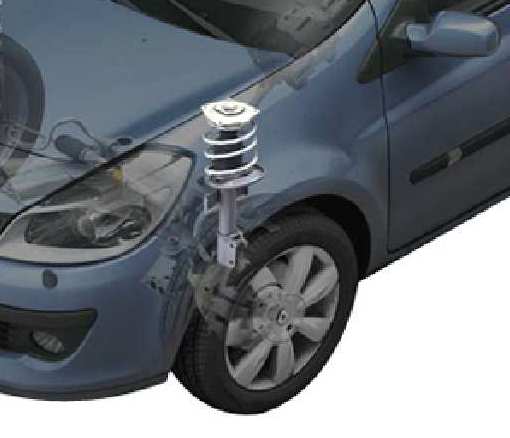
\includegraphics[height=2.5cm]{png/amort1} &&
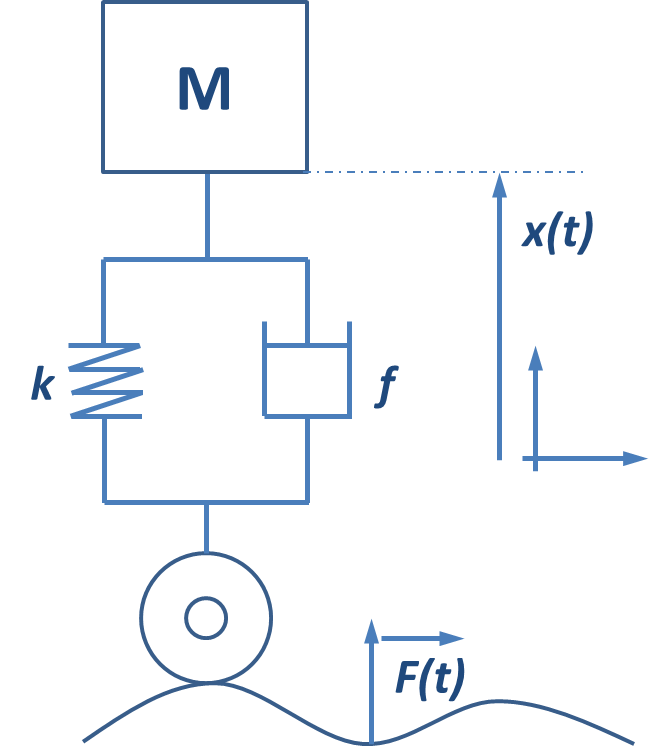
\includegraphics[height=3.5cm]{png/schema} && 
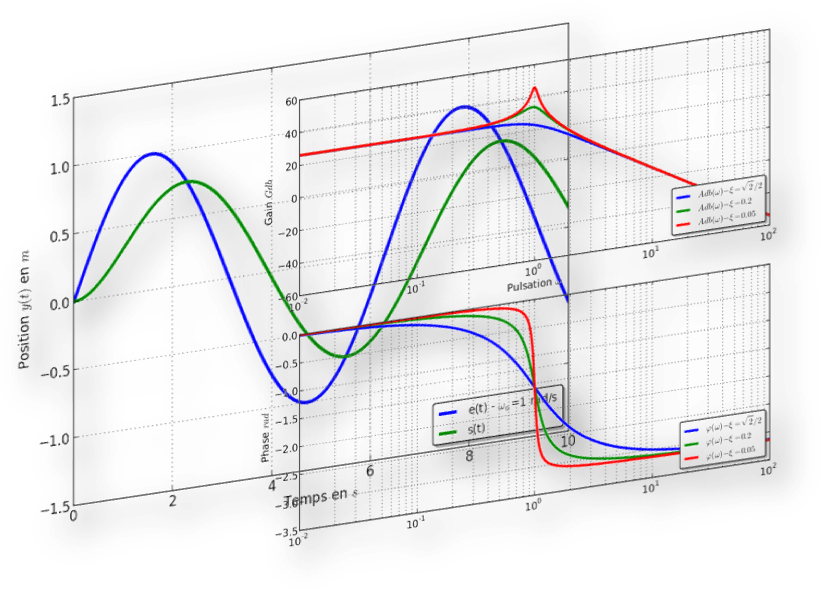
\includegraphics[height=3.5cm]{png/CourbesIntro}\\
\textit{Amortisseur d'un véhicule automobile} &&
\textit{Schématisation du mécanisme} &&
\textit{Réponses harmoniques}\\
%\textit{Schéma bloc } \\
\end{tabular}
\end{center}


\begin{savoir}
\textbf{Savoirs :}
\begin{itemize}
\item Rés.-C5 : Performances d'un système asservi
\begin{itemize}
\item Rés-C5-S2 : Tracer une réponse temporelle ou fréquentielle
\end{itemize}
\end{itemize}
\end{savoir}




\setlength{\parskip}{0ex plus 0.2ex minus 0ex}
 \renewcommand{\contentsname}{}
 \renewcommand{\baselinestretch}{1}

\tableofcontents

 \renewcommand{\baselinestretch}{1.2}
\setlength{\parskip}{2ex plus 0.5ex minus 0.2ex}

% \vspace{1cm}
\textit{Ce document évolue. Merci de signaler toutes erreurs ou coquilles.}



\section{Présentation}
\subsection{Caractérisation d'un signal sinusoïdal}

On peut définir un signal sinusoïdal sous la forme suivante :
$$
f(t)=A \sin(\omega \cdot t + \varphi)
$$
\begin{minipage}[c]{.45\linewidth}
et on note :
\begin{itemize}
\item $A$ : l'amplitude de la sinusoïde;
\item $\omega$ : la pulsation en $rad/s$;
\item $\varphi$ : la phase à l'origine en $rad$.
\end{itemize}
\end{minipage}\hfill
\begin{minipage}[c]{.45\linewidth}
On a par ailleurs :
\begin{itemize}
\item $T=\dfrac{2\pi}{\omega}$ : la période de la sinusoïde en $s$;
\item $f=\dfrac{1}{T}$ : fréquence de la sinusoïde en $Hz$.
\end{itemize}
\end{minipage}
\vspace{.5cm}

\begin{minipage}[c]{.3\linewidth}
\begin{center}
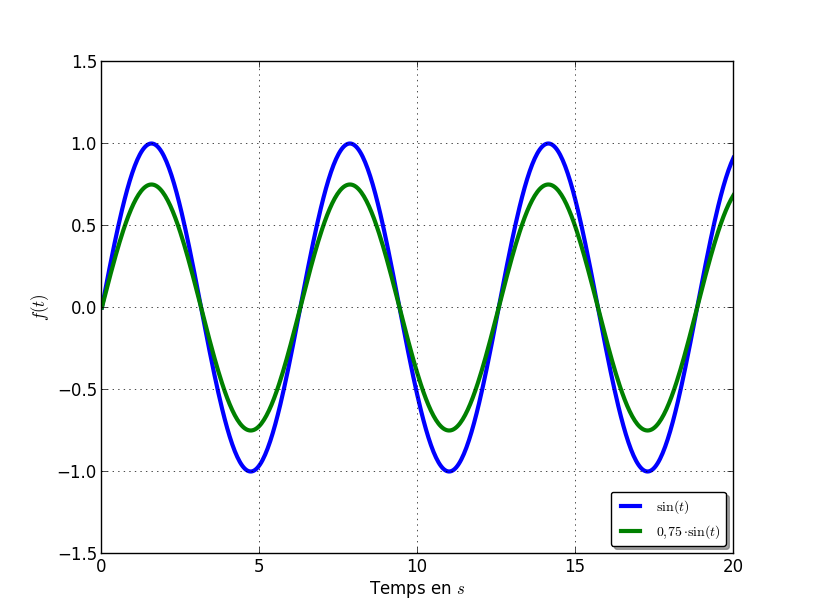
\includegraphics[width=.95\textwidth]{png/sinus_ampli}

\textit{Sinus amplifiés}
\end{center}
\end{minipage}\hfill
\begin{minipage}[c]{.3\linewidth}
\begin{center}
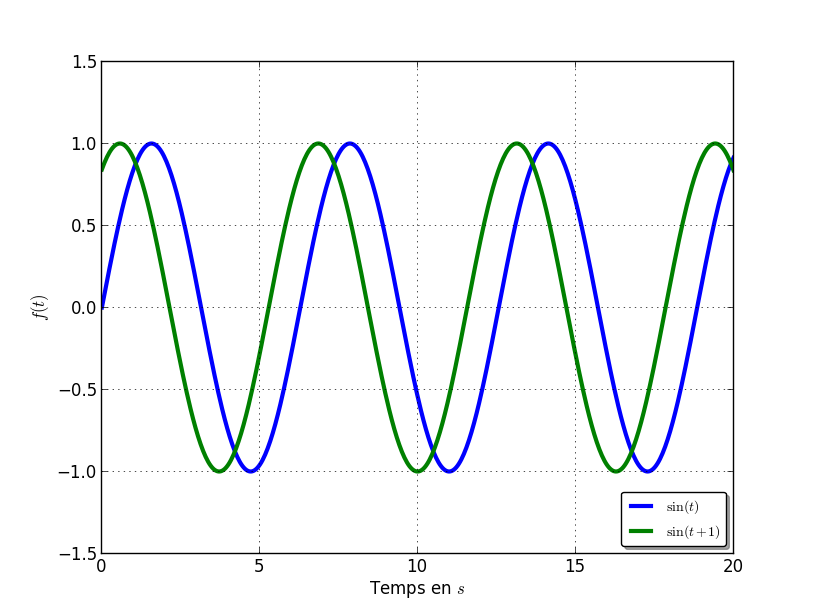
\includegraphics[width=.95\textwidth]{png/sinus_dephase}

\textit{Sinus déphasés}
\end{center}
\end{minipage}\hfill
\begin{minipage}[c]{.3\linewidth}
\begin{center}
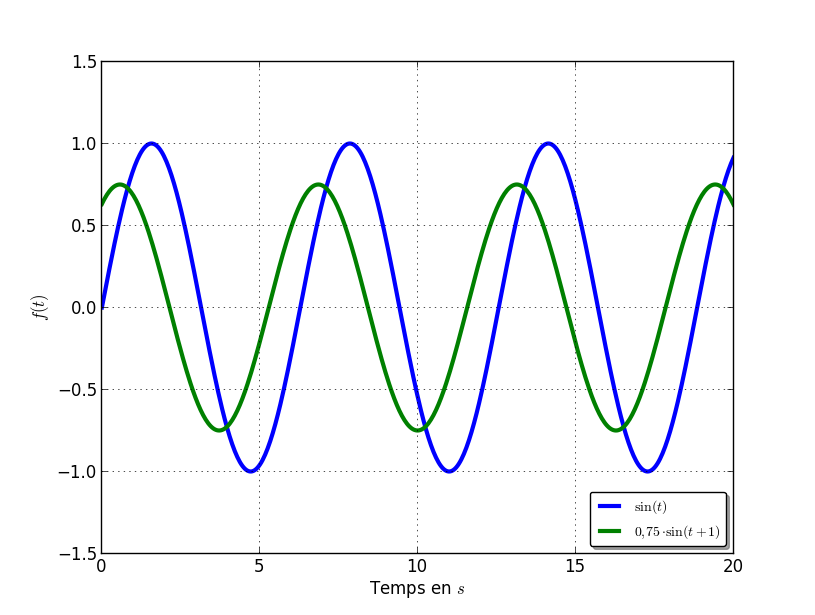
\includegraphics[width=.95\textwidth]{png/sinus_ampli_dephase}

\textit{Sinus amplifiés et déphasés}
\end{center}
\end{minipage}


\subsection{Réponse temporelle d'un système d'ordre 1 à une entrée sinusoïdale}

Soit un système du premier ordre de la forme $H(p)=\dfrac{1}{1+\tau p}$. Le gain de la fonction de transfert est donc de 1 et la constante de temps est de 1 seconde. 

Calculons la réponse temporelle $s(t)$ d'un premier ordre à une entrée sinusoïdale $e(t)=E_0  \sin \left( \omega_0 t\right)$. Dans le domaine de Laplace, on a $E(p)=E_0\dfrac{\omega_0}{\omega_0^2+p^2}$. $S(p)$ s'exprime donc sous la forme suivante :
$$
S(p)=E(p)\cdot H(p) = E_0\dfrac{\omega_0}{\omega_0^2+p^2} \cdot \dfrac{K}{1+\tau p }
= KE_0\omega_0 \left( \dfrac{1}{\omega_0^2+p^2} \cdot \dfrac{1}{1+\tau p }\right)
$$

En réalisant la transformée de Laplace inverse, on obtient : 
$$
s(t)=\dfrac{KE_0}{1+\tau^2\omega_0^2} 
\left( 
\tau \omega_0  e^{-\dfrac{t}{\tau}} 
-\tau \omega_0  \cos \left( \omega_0 t \right)
+\sin \left( \omega_0 t\right)
\right)
$$



\begin{defi}
\textbf{Réponse harmonique}

On appelle réponse harmonique la sortie d'un système lorsqu'il est soumis à une entrée sinusoïdale. Elle permet de caractériser le comportement dynamique du système.
\end{defi}



On donne les réponses temporelles pour plusieurs valeurs de la pulsation du signal d'entrée (\textbf{attention : les échelles des abscisses ne sont pas les mêmes sur chacune des figures}).

\begin{minipage}[c]{.24\linewidth}
\begin{center}
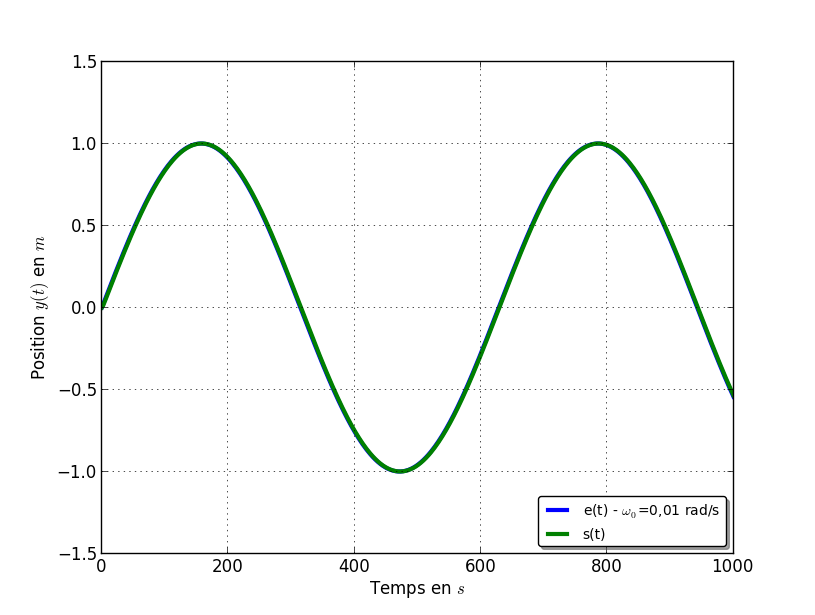
\includegraphics[width=\textwidth]{png/sinus_om001.png}

\textit{$\omega_0 =  0,01\; rad/s $ -- $T = 200 \pi \; s$}
\end{center}
\end{minipage}\hfill
\begin{minipage}[c]{.24\linewidth}
\begin{center}
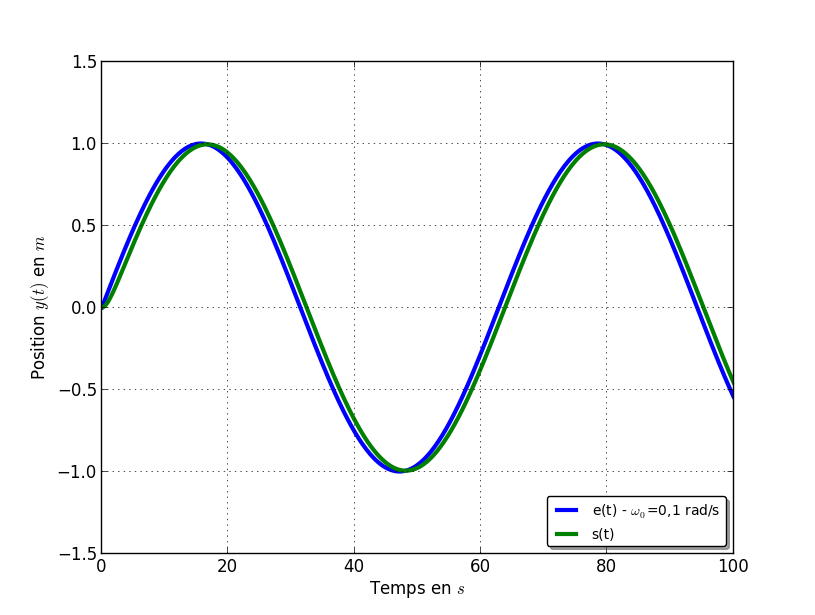
\includegraphics[width=\textwidth]{png/sinus_om01}
\textit{$\omega_0 =  0,1\; rad/s $ -- $ T = 20 \pi \; s$}
\end{center}
\end{minipage}\hfill
\begin{minipage}[c]{.24\linewidth}
\begin{center}
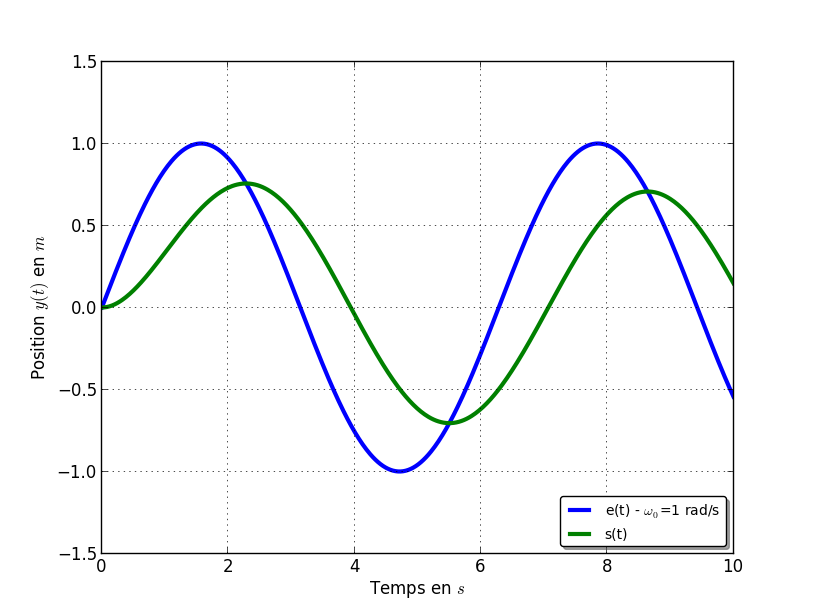
\includegraphics[width=\textwidth]{png/sinus_om1}

\textit{$\omega_0 =  1\; rad/s $ -- $ T = 2 \pi \; s$}
\end{center}
\end{minipage}\hfill
\begin{minipage}[c]{.24\linewidth}
\begin{center}
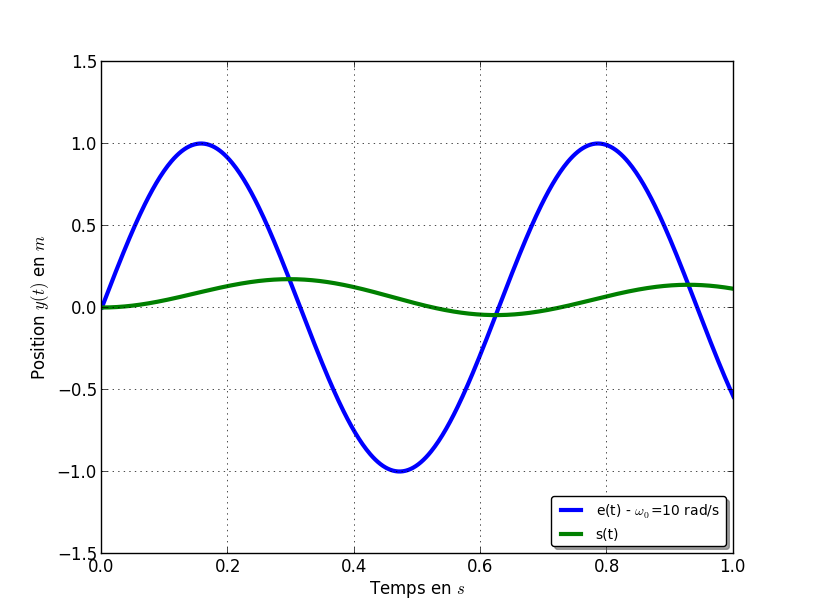
\includegraphics[width=\textwidth]{png/sinus_om10}

\textit{$\omega_0 =  10\; rad/s $ -- $ T = 0,2 \pi \; s$}
\end{center}
\end{minipage}

On constate que quand la pulsation du signal augmente, on observe un déphasage entre le signal d'entrée et le signal de sortie ainsi qu'une atténuation du signal de sortie. 

\section{Diagrammes de Bode}

\subsection{Calcul complexe}
Lorsque le système est soumis à une entrée sinusoïdale, la variable de la Laplace $p$ est substituée par $j\omega$. $H(j\omega)$ est appelée réponse en fréquence ou réponse harmonique du système.

\begin{resultat}
On rappelle que si $H(j\omega) = \dfrac{x_1+jy_1}{x_2+jy_2}$, alors : 
\begin{itemize}
\item on appelle $A(\omega)=|H(j\omega)|$ le module de $H$ (ou le gain de $H$) et on a : 
$$
A(\omega)= \dfrac{\sqrt{x_1^2+y_1^2}}{\sqrt{x_2^2+y_2^2}}
$$
\item on appelle $\varphi(\omega)=Arg(H(j\omega))$ l'argument de $H$ (ou la phase de $H$) et on a : 
$$
\varphi(\omega)= \arctan \dfrac{y_1}{x_1}-\arctan \dfrac{y_2}{x_2}
$$
\end{itemize}
\end{resultat}

\begin{rem}
On appelle $AdB$ le gain en décibel et on a :
$$
AdB(\omega)=20 \log A(\omega)
$$
\end{rem}

\begin{exemple}
Soit $H(p)$ une fonction de transfert d'ordre 1 :
$$
H(j\omega)= \dfrac{K}{1+\tau j\omega }
$$

On a alors : 
$$
AdB(\omega) = 20 \log \left(\dfrac{\sqrt{K^2}}{\sqrt{1^2+(\tau\omega)^2}}\right) = 20 \log K - 10 \log \left(1+\tau^2\omega^2 \right)
$$
$$
\varphi(\omega)= \arctan \dfrac{0}{K}-\arctan \dfrac{\tau\omega}{1} = - \arctan \tau\omega
$$

\end{exemple}

\subsection{Définition}

\begin{defi}
\textbf{Diagrammes de Bode}

Les diagrammes de Bode représentent deux courbes sur deux diagrammes distincts dans des repère semi logarithmiques :
\begin{itemize}
\item la courbe de gain en décibel en fonction de la pulsation $\omega$;
\item la courbe de phase (en degrés ou radians) en fonction de la pulsation $\omega$.
\end{itemize}

\end{defi}

\subsubsection{Tracé des diagrammes de Bode}
Le tracé de Bode comprend toujours le diagramme de gain superposé avec le diagramme de phase. Dans le cas d'un système du premier ordre, la représentation directe du diagramme de Bode serait la suivante.


On remarque de fortes variations de la courbe lorsque $\omega$ est petit. En conséquences, on choisit usuellement de représenter les diagrammes de Bode dans un repère semi logarithmique. 

\begin{minipage}[c]{.48\linewidth}
\begin{center}
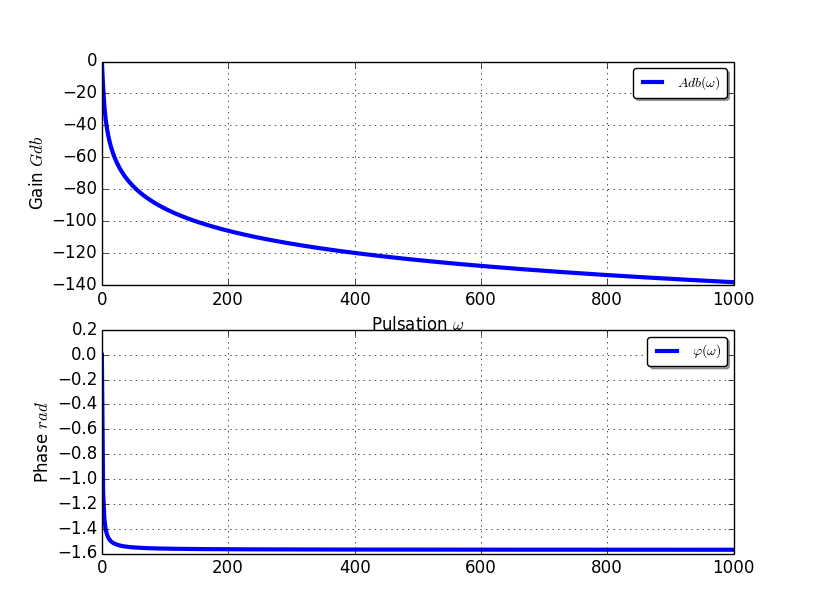
\includegraphics[width=\textwidth]{png/bode_orth}
\end{center} 
\end{minipage}\hfill
\begin{minipage}[c]{.48\linewidth}
\begin{center}
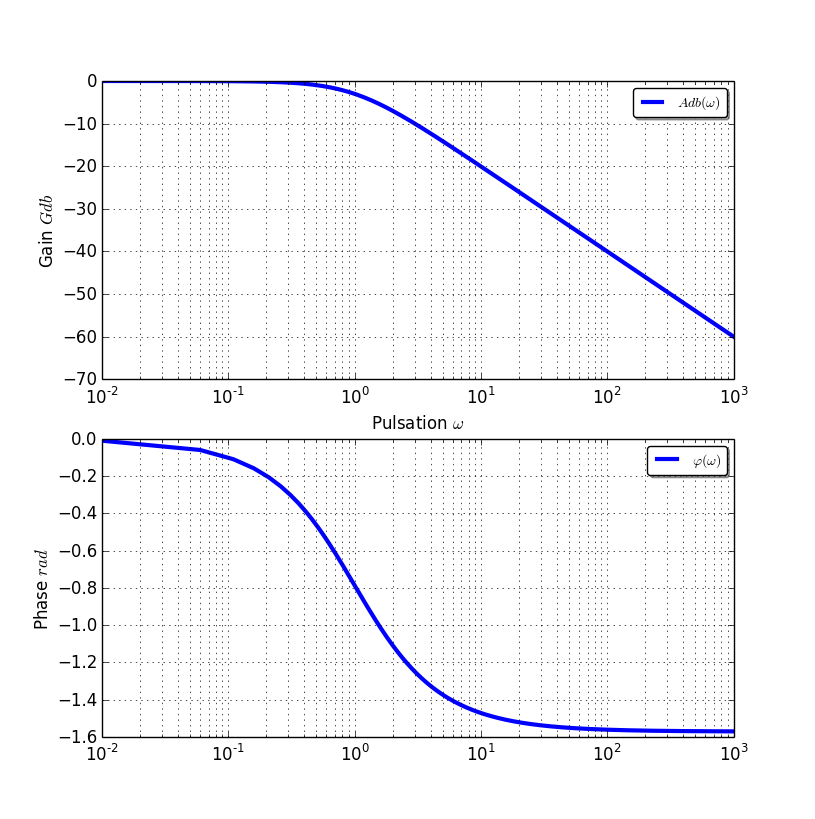
\includegraphics[width=\textwidth]{png/bode_semilog}
\end{center}
\end{minipage} 
 
\subsubsection{Lien entre la réponse temporelle et le diagramme de Bode}
Une réponse temporelle pour une pulsation donnée permet de tracer un point dans la courbe de gain et un point dans la courbe de phase.
\begin{center}
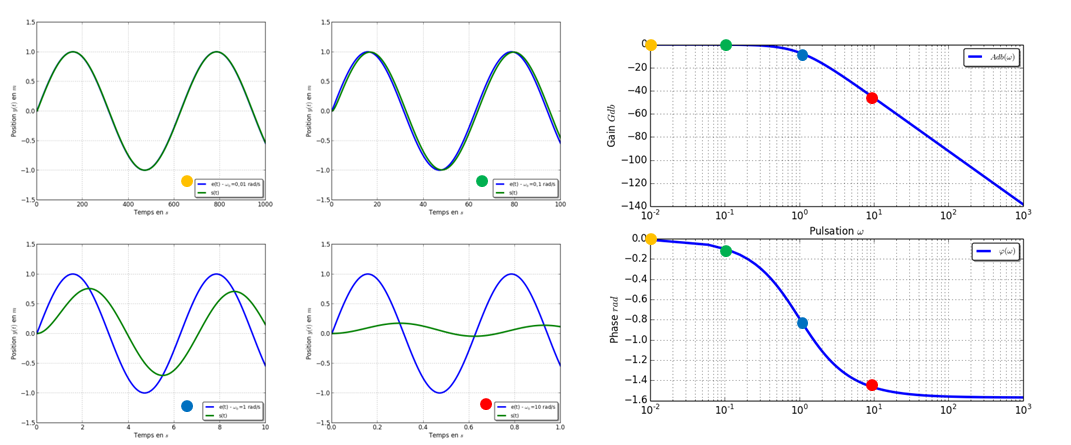
\includegraphics[width=\textwidth]{png/temp_bode}
\end{center}

\begin{center}
\begin{tabular}{|c|c|c|c|c|}
\hline
Pulsation ($rad/s$) & 0,01 & 0,1 & 1 & 10\\
\hline
Rapport des amplitudes & 1 & 1 & 0,756 & 0,17 \\
\hline
Décalage temporel ($s.$) & 0 & 0 &0,721  &0,14  \\
\hline
Gain ($dB$) & 0 & 0 & -2,43 %-6,93
& -15,39 % -46,15
\\
\hline
Déphasage ($rad$) & 0 & 0 & 0,72 & 1,4\\
\hline
\end{tabular}
\end{center}
% 1  rad/s >> T = 2pi      = 6,28    6,28 s <> 2pi rad => 0,721 <> 
% 10 rad/s >> T = 2pi/10 = 0,628  0,628s <> 2pi      => 0,14 <> 1,4 rad
% 


\begin{resultat}
La représentation de la \textbf{fonction de transfert} dans les diagrammes de Bode permet d'avoir des informations sur la comportement du système. 

Attention, suivant les cas, il sera nécessaire de représenter la FTBO \textbf{ou} la FTBF.
\end{resultat}
\subsection{Représentation d'un système asservi}

Généralement, une fonction de transfert s'écrit sous la forme d'un produit de fonction rationnelles. Ainsi, notons $H(j\omega)=F(j\omega) \cdot G(j\omega)$. 

On montre que le gain décibel de $H$ est sous la forme :
$$
AdB(\omega) = 20 \log |F(j\omega) |+20 \log |G(j\omega) |
$$

et que la phase est sous la forme :
$$
Arg(\omega) = Arg \left(F(j\omega) \right)+Arg \left(G(j\omega) \right)
$$

Ainsi pour tracer le gain et la phase d'une fonction de transfert s'exprimant sous la forme de produit de fonctions de transfert élémentaire, il suffit de tracer les fonctions de transfert élémentaire dans les diagrammes de Bode puis de les sommer.

\section{Réponse harmonique d'un gain}

\begin{minipage}[c]{.48\linewidth}
\begin{center}
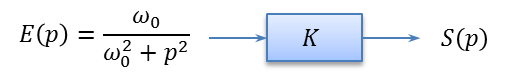
\includegraphics[width=.9\textwidth]{png/gain_bloc}
\end{center}

Ici $H(j\omega)=K$. On a :
\begin{itemize}
\item [$\bullet$] $AdB(\omega)=20 \log K$;
\item [$\bullet$] $\varphi(\omega)= \arctan \dfrac{0}{K} = 0$.
\end{itemize}
\end{minipage}\hfill
\begin{minipage}[c]{.48\linewidth}
\begin{center}
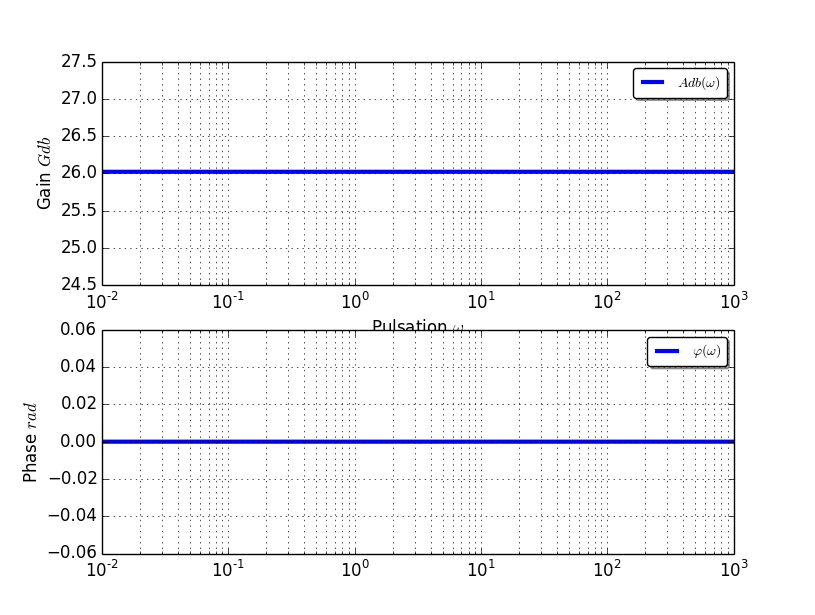
\includegraphics[width=.9\textwidth]{png/gain_bode}

\textit{Diagramme de Bode -- $H(p)=20$}
\end{center}
\end{minipage}


\section{Réponse harmonique d'un intégrateur}

\subsection{Réponse harmonique d'un intégrateur}
\begin{minipage}[c]{.48\linewidth}
\begin{center}
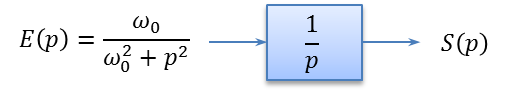
\includegraphics[width=.9\textwidth]{png/integrateur_bloc}
\end{center}

Ici $H(j\omega)=\dfrac{1}{j\omega}=-\dfrac{j}{\omega}$. On a :
\begin{itemize}
\item [$\bullet$] $AdB(\omega)=20 \log \dfrac{1}{\omega}=-20\log \omega$;
\item [$\bullet$] $\varphi(\omega)= \arctan \dfrac{\dfrac{-1}{\omega}}{0}$ tend vers $-\dfrac{\pi}{2}$.
\end{itemize}

\end{minipage}\hfill
\begin{minipage}[c]{.48\linewidth}
\begin{center}
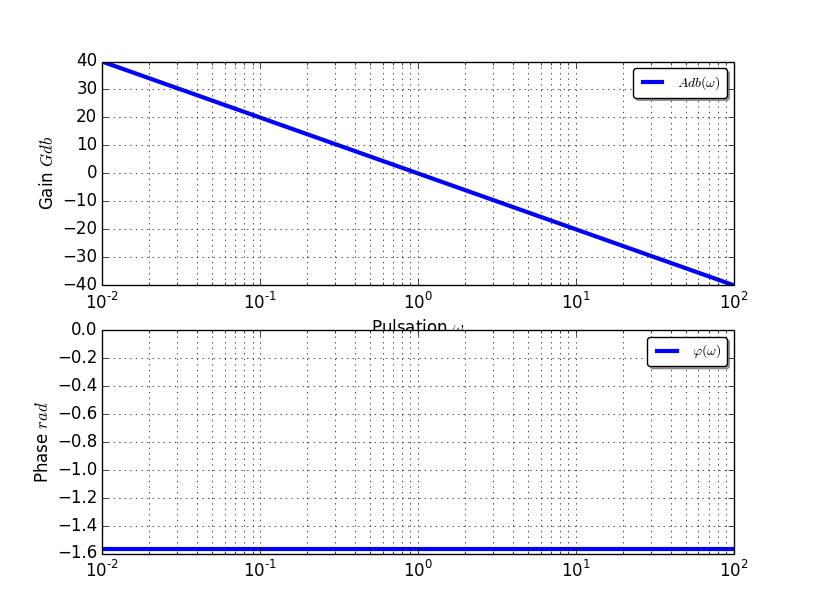
\includegraphics[width=.9\textwidth]{png/integrateur_bode}

\textit{Diagramme de Bode -- $H(p)=\dfrac{1}{p}$}
\end{center}
\end{minipage}

\subsection{Réponse harmonique système proportionnel intégral}
\begin{minipage}[c]{.48\linewidth}
\begin{center}
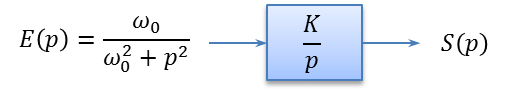
\includegraphics[width=.9\textwidth]{png/proportionnel_integral_bloc}
\end{center}
Ici $H(j\omega)=\dfrac{K}{j\omega}=-\dfrac{j}{\omega}$. On a :
\begin{itemize}
\item [$\bullet$] $AdB(\omega)=20 \log \dfrac{K}{\omega}=20\log K -20\log \omega$;
\item [$\bullet$] $\varphi(\omega)= \arctan \dfrac{\dfrac{-K}{\omega}}{0}$ tend vers $-\dfrac{\pi}{2}$.
\end{itemize}
\end{minipage}\hfill
\begin{minipage}[c]{.48\linewidth}
\begin{center}
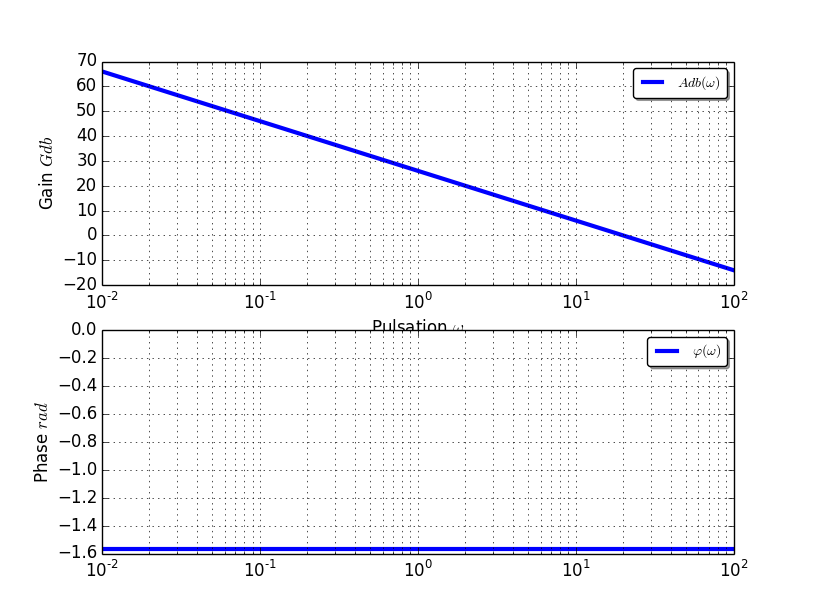
\includegraphics[width=.9\textwidth]{png/proportionnel_integral_bode}

\textit{Diagramme de Bode -- $H(p)= \dfrac{20}{p}$}
\end{center}
\end{minipage}

\subsection{Réponse harmonique d'un dérivateur}
\begin{minipage}[c]{.48\linewidth}
\begin{center}
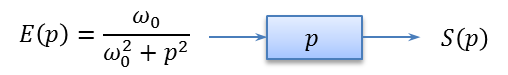
\includegraphics[width=.9\textwidth]{png/derivateur_bloc}
\end{center}

Ici $H(j\omega)= j\omega$. On a :
\begin{itemize}
\item [$\bullet$] $AdB(\omega)=20 \log {\omega}=20\log \omega$;
\item [$\bullet$] $\varphi(\omega)= \arctan \dfrac{\dfrac{1}{\omega}}{0}$ tend vers $\dfrac{\pi}{2}$.
\end{itemize}

\end{minipage}\hfill
\begin{minipage}[c]{.48\linewidth}
\begin{center}
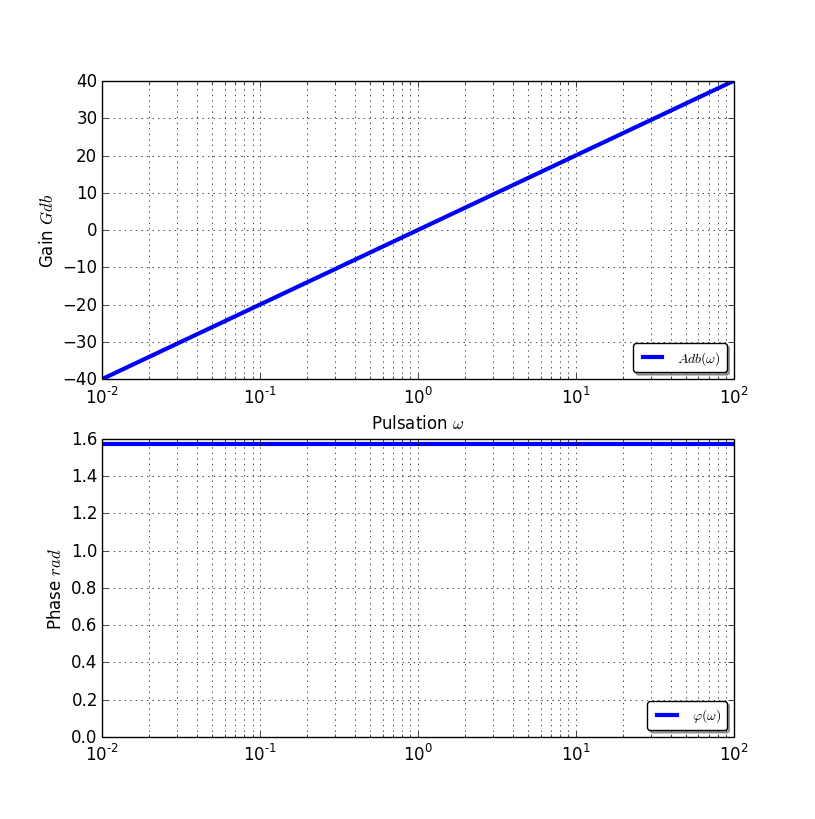
\includegraphics[width=.9\textwidth]{png/derivateur_bode}

\textit{Diagramme de Bode -- $H(p)=p$}
\end{center}
\end{minipage}

\section{Réponse harmonique d'un système du premier ordre}

\subsection{Tracé réel}
\begin{minipage}[c]{.48\linewidth}
\begin{center}
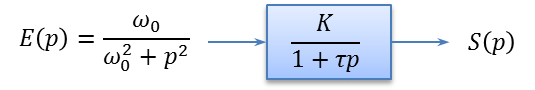
\includegraphics[width=.9\textwidth]{png/ordre1_bloc}
\end{center}

On a $H(j\omega)=\dfrac{K}{1+j\omega p}$. Calculons le gain de la fonction de transfert :
$$
AdB(\omega) 
= 20\log \left(\dfrac{ \sqrt{ K^2} }{\sqrt{1+\tau^2\omega^2}}\right)
= 20\log K - 10 \log \left( 1+\tau^2\omega^2\right)
$$

$$
\varphi(\omega) 
= \arctan\left( \dfrac{0}{K}\right)-\arctan\left( \dfrac{\tau\omega}{1}\right)
= -\arctan\tau\omega
$$
\end{minipage}\hfill
\begin{minipage}[c]{.48\linewidth}
\begin{center}
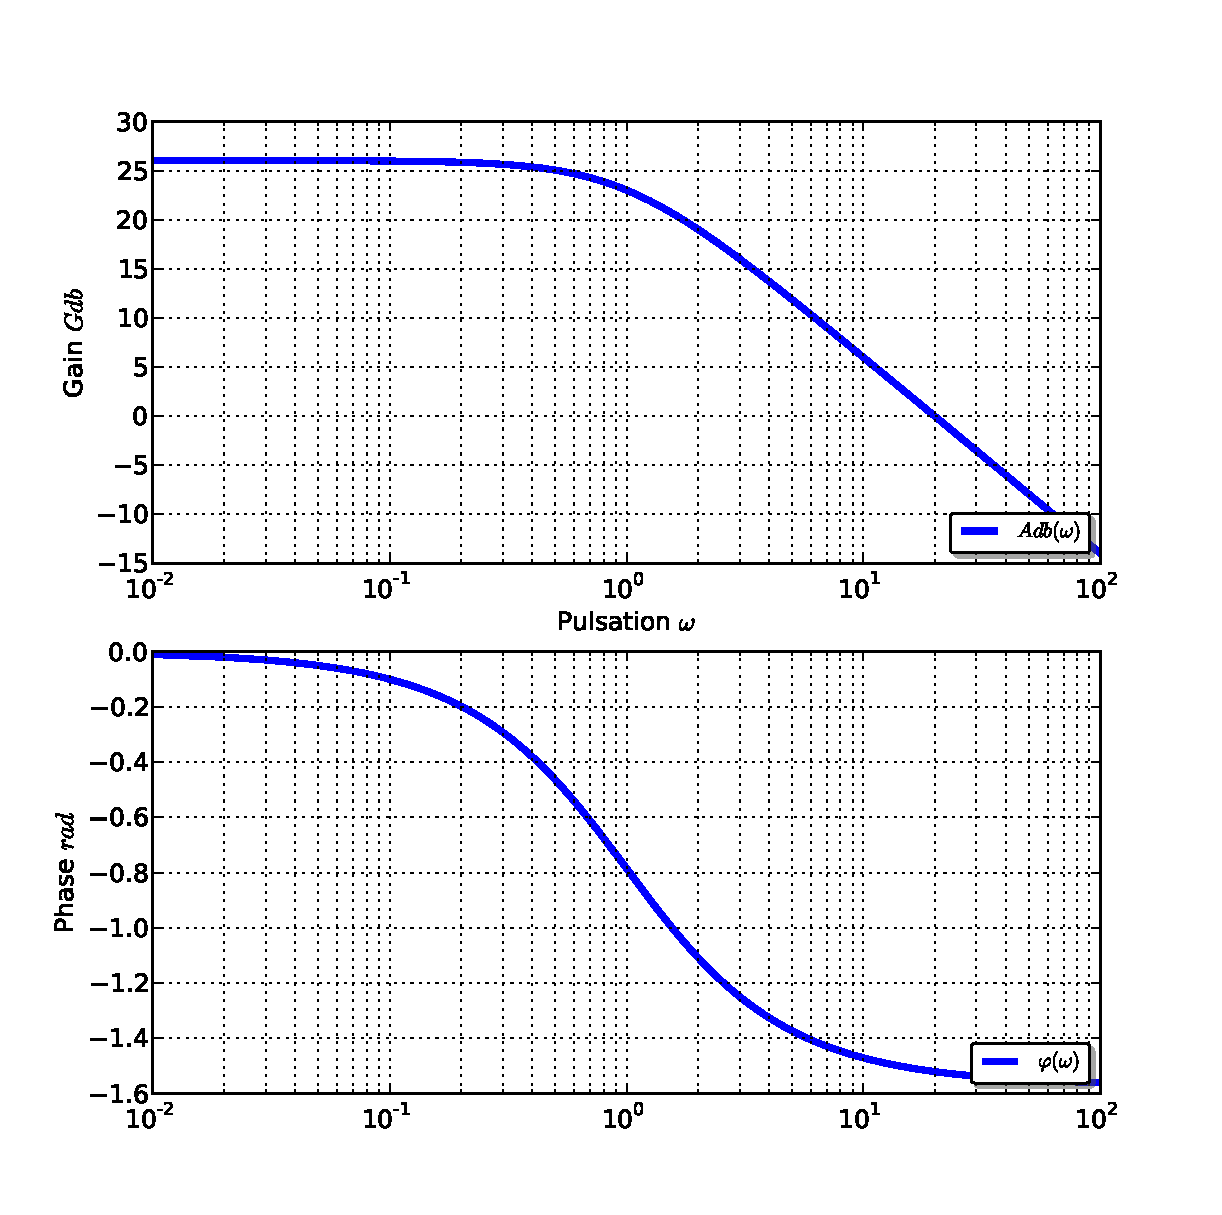
\includegraphics[width=.9\textwidth]{png/ordre1_bode}

\textit{Diagramme de Bode -- $H(p)=\dfrac{20}{1+p}$}
\end{center}
\end{minipage}

\subsection{Tracé asymptotique}
\paragraph*{En 0}
Pour le gain, on a $\underset{\omega \to 0 }{\lim} AdB(\omega) = 20 \log K$. Lorsque $\omega$ tend vers 0, $AdB(\omega)$ tend vers une constante, ce qui donne une droite horizontale.

Pour la phase, on a $\underset{\omega \to 0 }{\lim} \varphi(\omega) = 0$. Lorsque $\omega$ tend vers 0, $\varphi(\omega)$ tend vers une constante, ce qui donne une droite horizontale.

\paragraph*{En $+\infty$}
Pour le gain, on a $+\infty $ : $AdB(\omega) = 20 \log K -20\log \tau-20\log \omega = 20 \log \dfrac{K}{\tau} -20\log \omega$. Cela correspond, dans un diagramme semi logarithmique à une droite passant par $20 \log \dfrac{K}{\tau}$ en $\omega=1$ et une pente de -20 $dB$ par décade. 

Pour la phase, on a $\underset{\omega \to +\infty }{\lim} \varphi(\omega) = -\dfrac{\pi}{2}$. Lorsque $\omega$ tend vers 0, $\varphi(\omega)$ tend vers une constante, ce qui donne une droite horizontale.

\paragraph*{Remarques}
L'intersection des deux asymptotes se détermine en cherchant $\omega$ tel que  $ 20 \log K = 20 \log \dfrac{K}{\tau} -20\log \omega \Longleftrightarrow 
20 \log T = -20\log \omega \Longleftrightarrow  \omega = \dfrac{1}{\tau}$.

\begin{resultat}
Les asymptotes s'intersectent en $\omega = \dfrac{1}{\tau}$.
\end{resultat}

Calculons la valeur du gain au passage de $\omega = \dfrac{1}{\tau}$ :
$$
AdB\left(\dfrac{1}{\tau}\right) 
= 20\log K - 20 \log \sqrt{ 1+1} \simeq 20\log K - 3 
$$

On a donc une atténuation de $-3\,dB$ en $\omega = \dfrac{1}{\tau}$.

Par ailleurs, 
$$
\left|H\left(j\dfrac{1}{\tau}\right)\right| = \left|\dfrac{K}{1+j}\right| = \dfrac{K}{\sqrt{2}} = K\dfrac{\sqrt{2}}{2}
$$

\begin{warn}
Une atténuation de $-3\; dB$ n'est pas anodine. Elle correspond à une atténuation du signal de près de 30\% en régime permanent.
\end{warn}


Il est possible de calculer la pulsation pour laquelle l'asymptote oblique coupe l'axe des abscisses. Pour cela, il faut résoudre l'équation
$ 20 \log \dfrac{K}{\tau} -20\log \omega = 0$.
On a alors 
$$ 20\log \omega =  20 \log \dfrac{K}{\tau} \Longleftrightarrow \omega =  { \dfrac{K}{\tau}} $$

\begin{center}
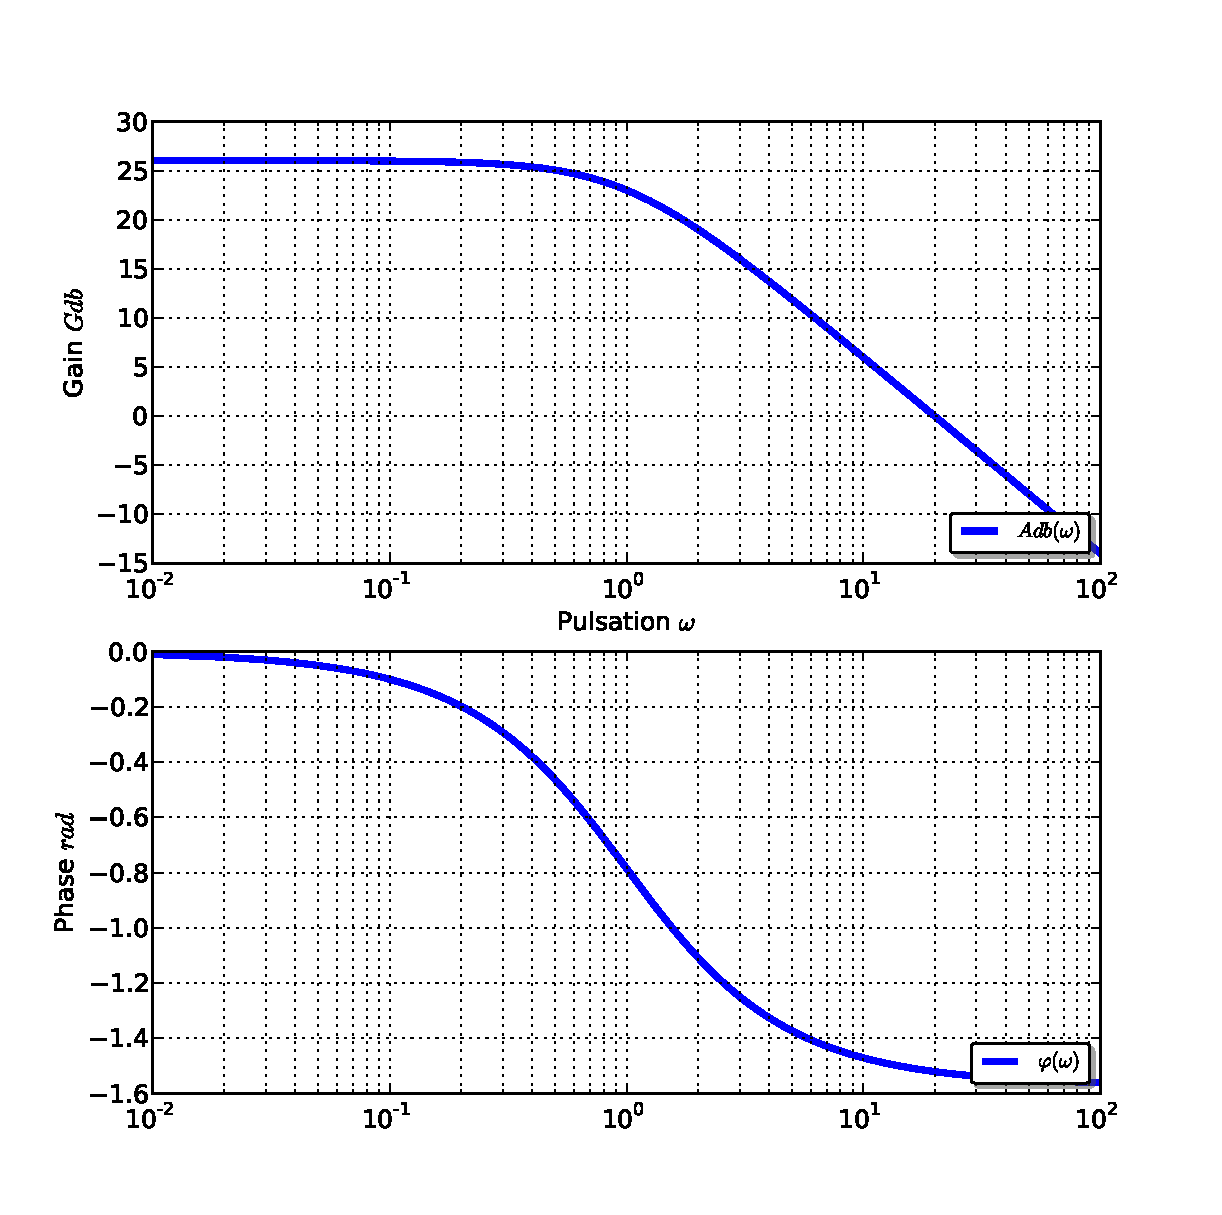
\includegraphics[width=.7\textwidth]{png/ordre1_bode.pdf}

\textit{Représentation asymptotique et tracé réel}
\end{center}

\section{Réponse harmonique d'un système du second ordre}

\begin{minipage}[c]{.48\linewidth}
\begin{center}
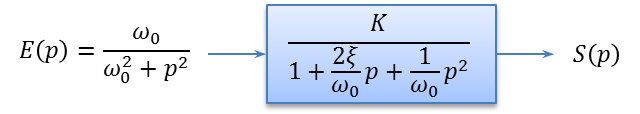
\includegraphics[width=.9\textwidth]{png/ordre2_bloc}
\end{center}
\end{minipage}\hfill
\begin{minipage}[c]{.48\linewidth}
\begin{center}
%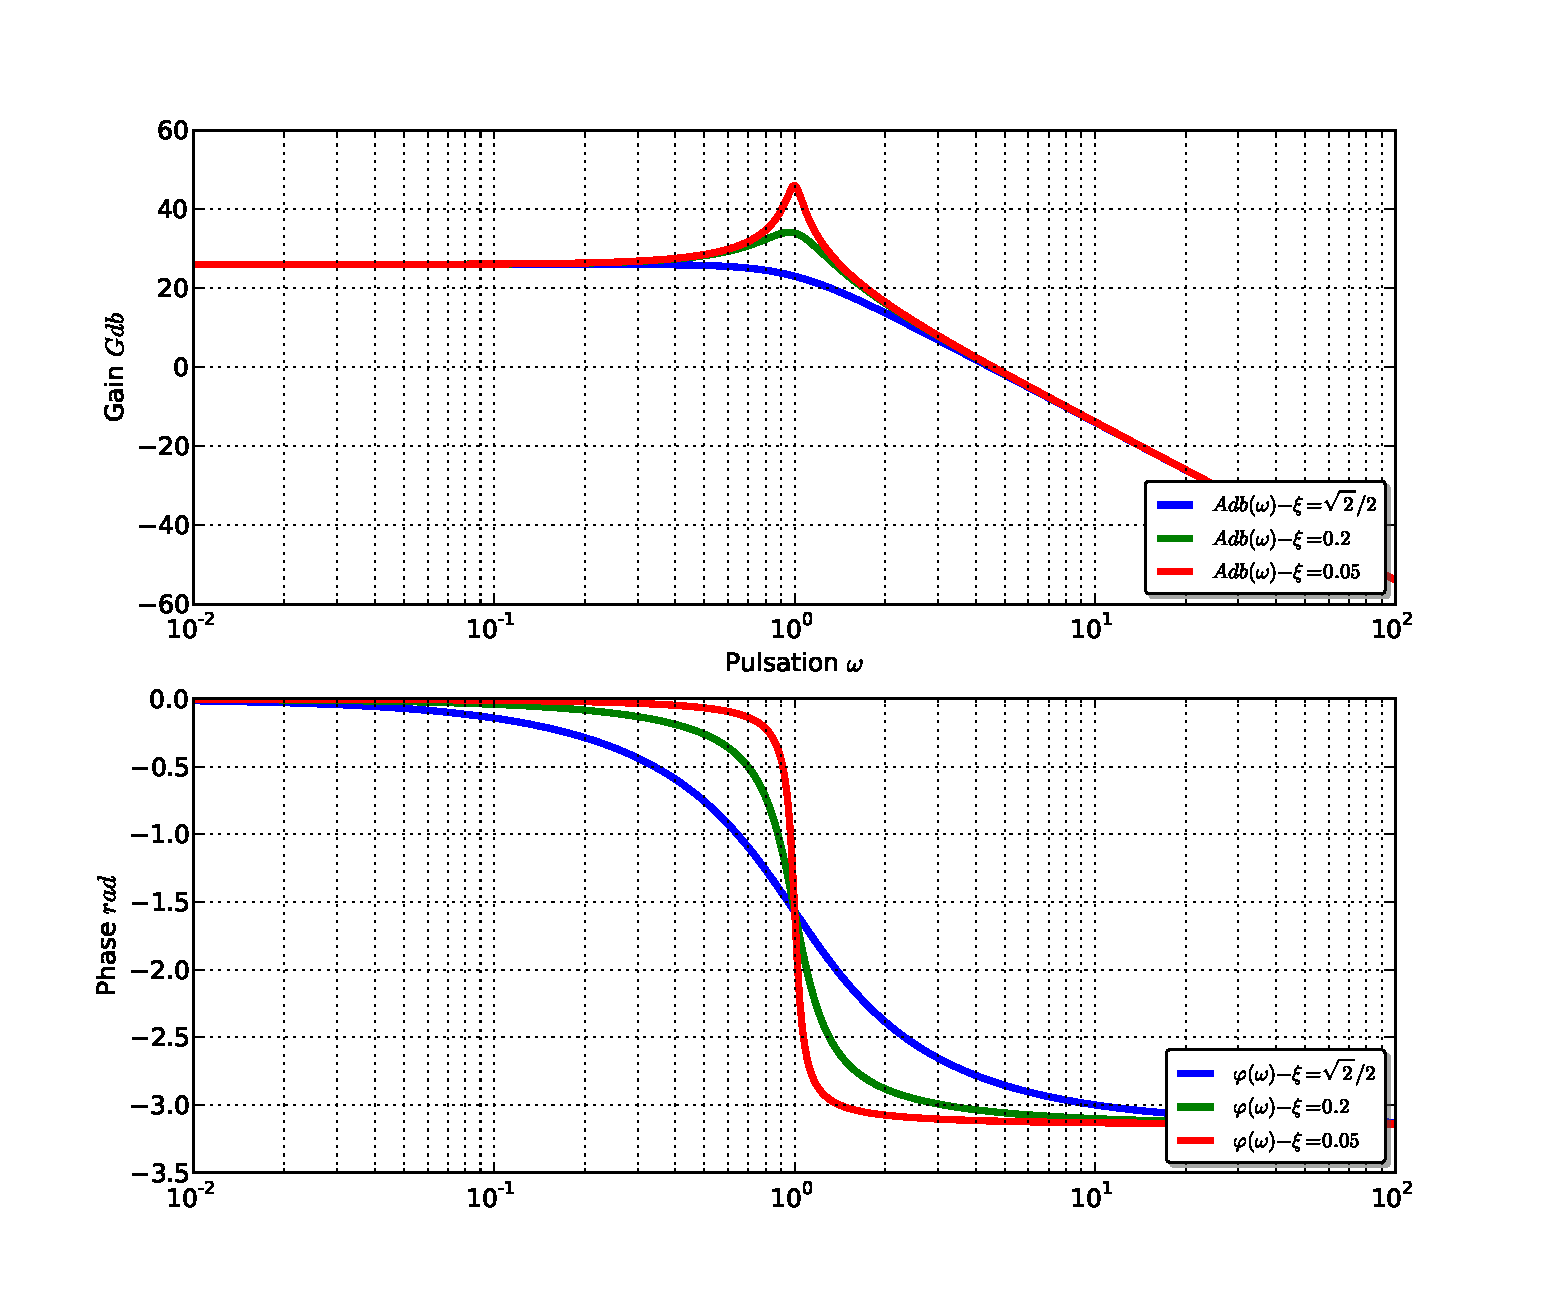
\includegraphics[width=.9\textwidth]{png/ordre2_bode}

%\textit{Diagramme de Bode -- $H(p)=$}
\end{center}
\end{minipage}

\subsection{Cas où $\xi\geq1$}
%\begin{minipage}[c]{.48\linewidth}
Dans ce cas, le dénominateur de la fonction de transfert peut se factoriser sous la forme :
$H(p)=\dfrac{K}{\left(1+\tau_1 p \right)\left(1+\tau_2 p \right)}$.

Le tracé de cette fonction de transfert revient à tracer les diagrammes de Bode des fonctions de transfert suivantes :
\begin{itemize}
\item $H_1(p)=K$;
\item $H_2(p)=\dfrac{1}{1+\tau_1 p }$;
\item $H_3(p)=\dfrac{1}{1+\tau_2 p }$.
\end{itemize}

On peut alors sommer les 3 fonctions de transfert. 

Tracer le diagramme de Bode asymptotique de la fonction de transfert 
$H(p)=\dfrac{20}{\left(1+ p \right)\left(1+10 p \right)}$.

\begin{center}
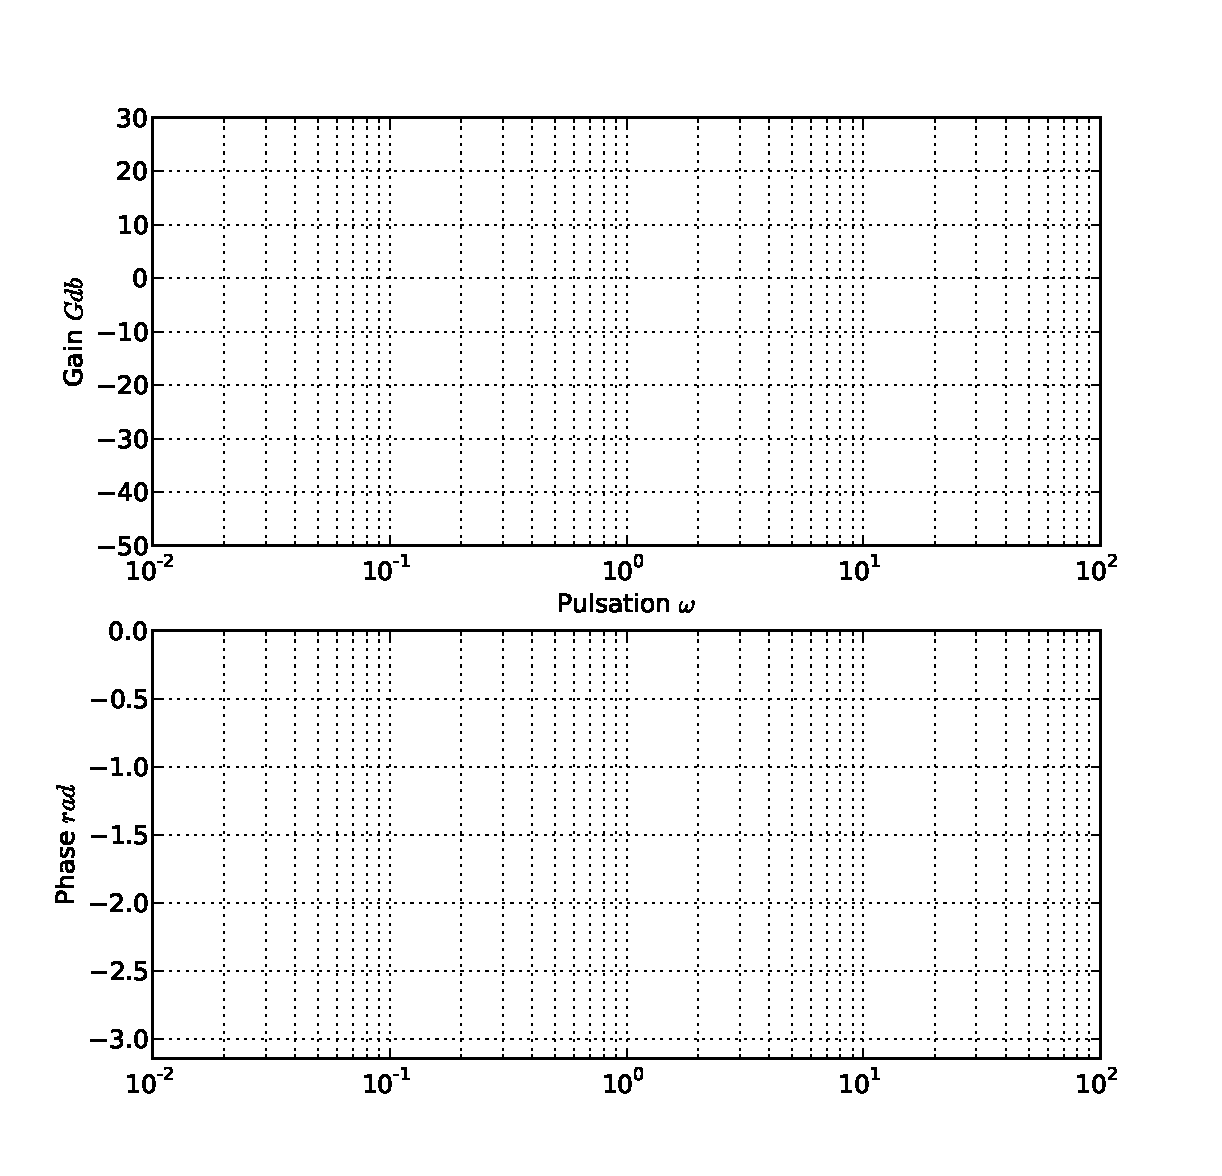
\includegraphics[width=.8\textwidth]{png/bode_vierge.pdf}

\textit{Diagramme de Bode -- $H(p)=\dfrac{20}{\left(1+ p \right)\left(1+10 p \right)}$}
\end{center}

%\end{minipage}\hfill
%\begin{minipage}[c]{.48\linewidth}
%\begin{center}
%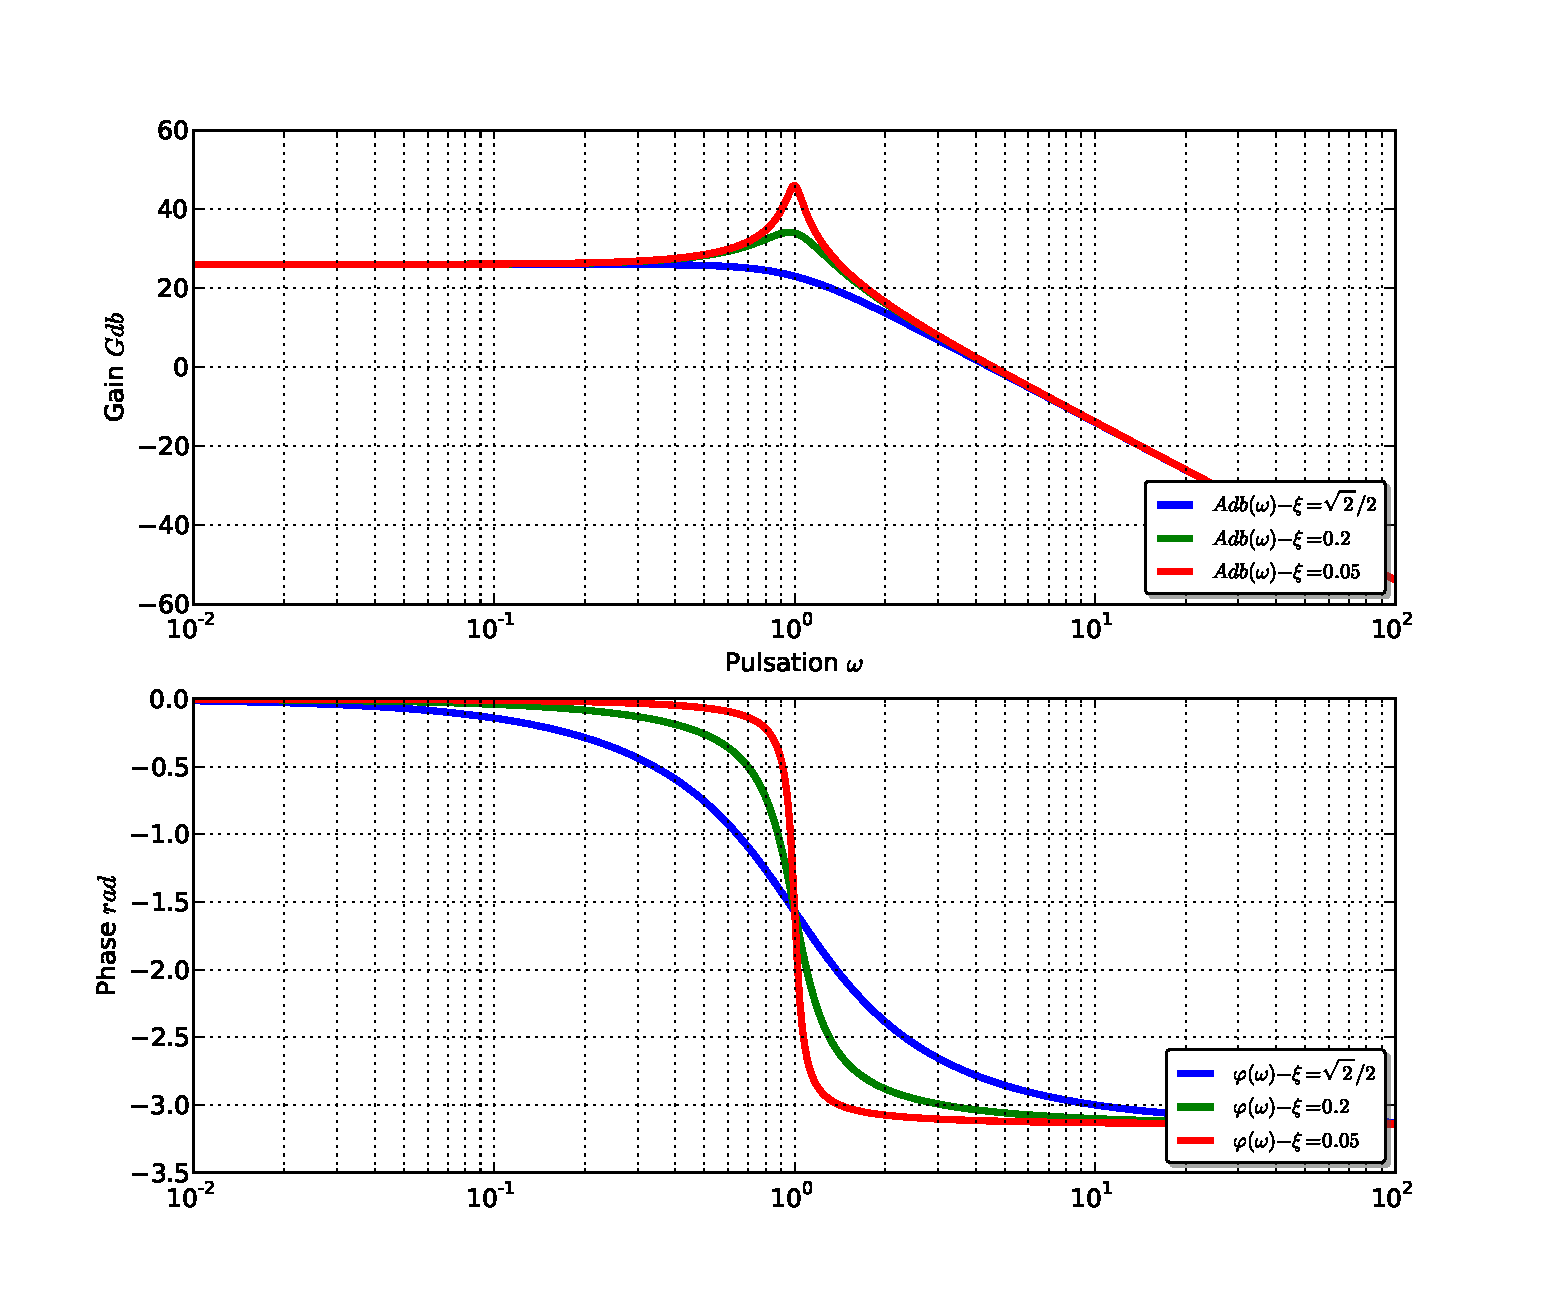
\includegraphics[width=.9\textwidth]{png/ordre2_bode}

%\textit{Diagramme de Bode -- $H(p)=$}
%\end{center}
%\end{minipage}


%\subsection{Cas où $\xi=1$}
%%\begin{minipage}[c]{.48\linewidth}
%Dans ce cas, le dénominateur de la fonction de transfert peut se factoriser sous la forme :
%$H(p)=\dfrac{K}{\left(1+\tau p \right)^2}$.
%
%Tracer le diagramme de Bode asymptotique de la fonction de transfert 
%$H(p)=\dfrac{20}{\left(1+ p \right)^2}$.
%
%\begin{center}
%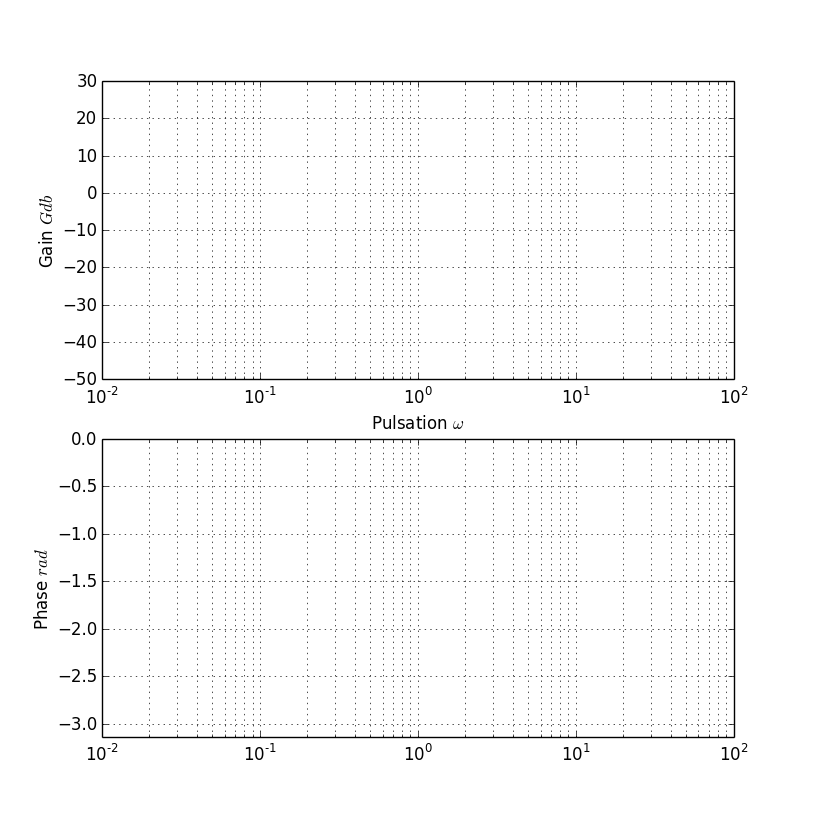
\includegraphics[width=.9\textwidth]{png/bode_vierge}
%
%\textit{Diagramme de Bode -- $H(p)=\dfrac{20}{\left(1+ p \right)^2}$}
%\end{center}
%
%%\end{minipage}\hfill
%%\begin{minipage}[c]{.48\linewidth}
%%\begin{center}
%%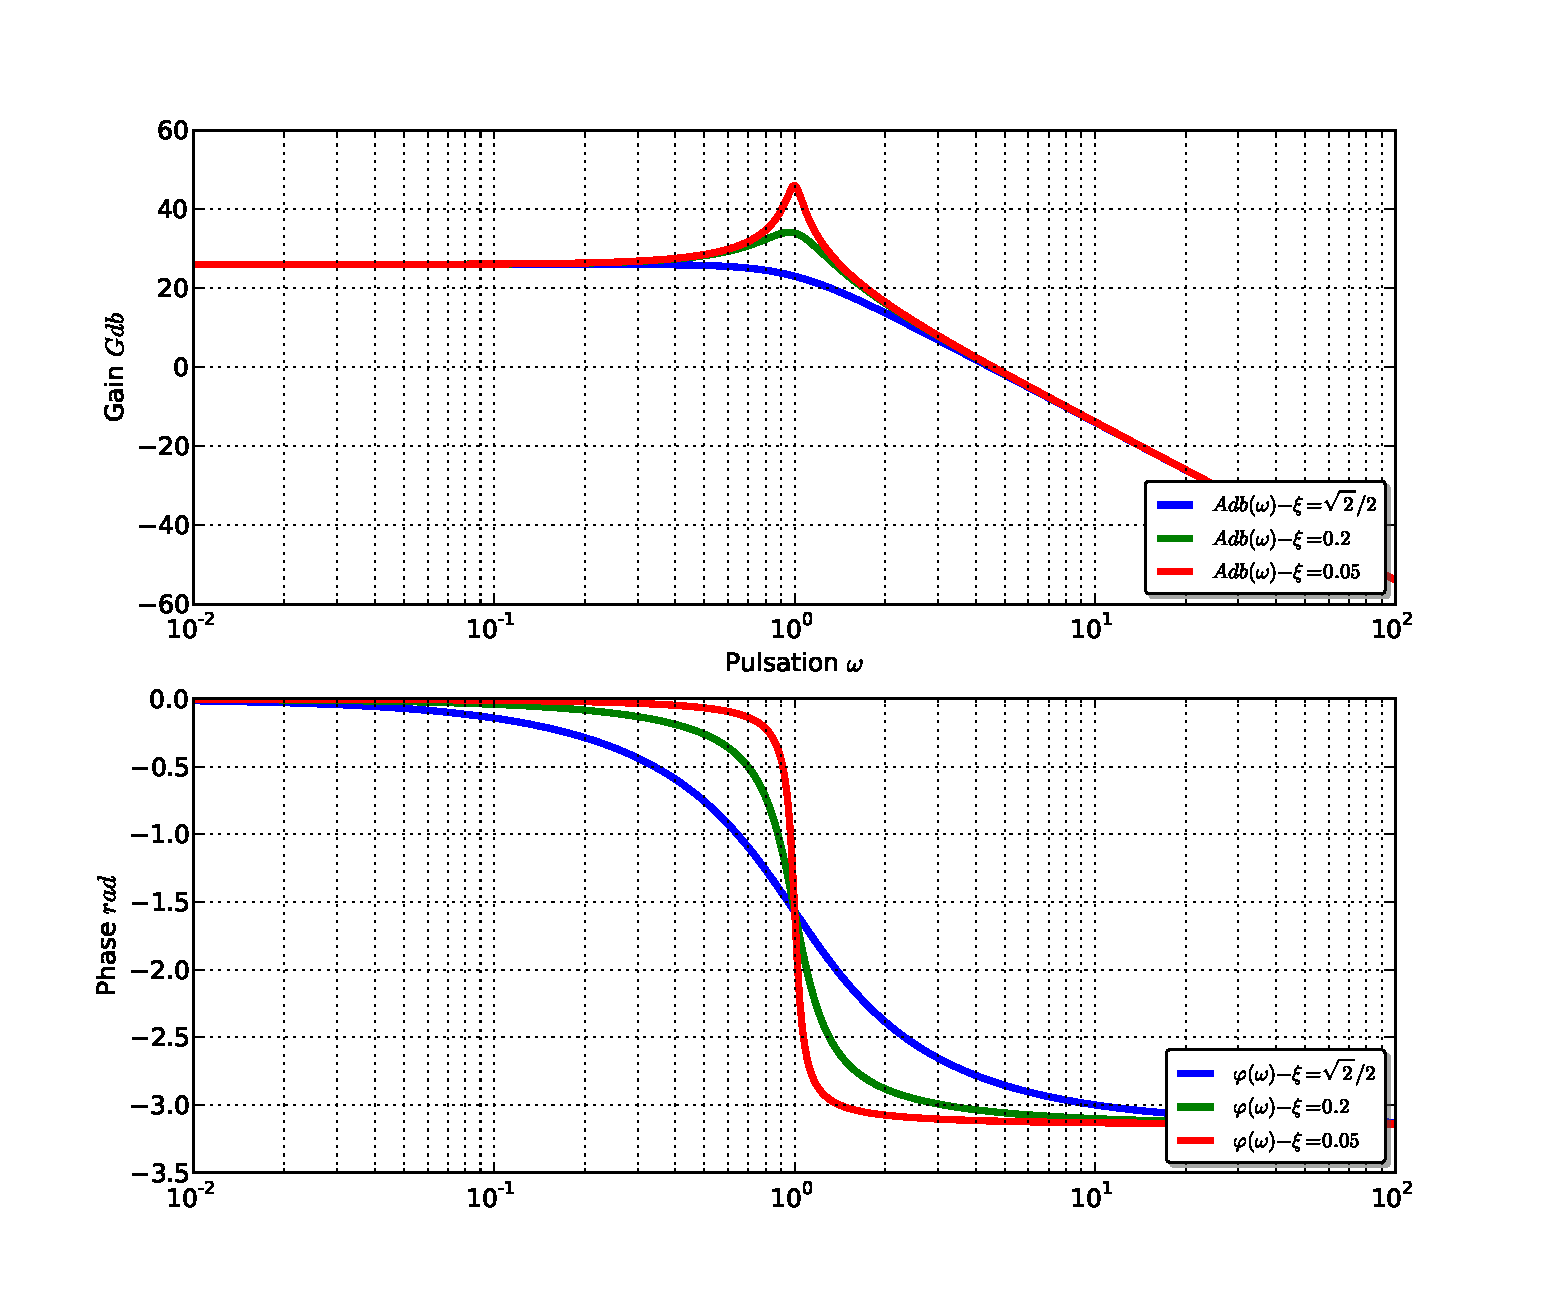
\includegraphics[width=.9\textwidth]{png/ordre2_bode}
%
%%\textit{Diagramme de Bode -- $H(p)=$}
%%\end{center}
%%\end{minipage}

\subsection{Cas où $\xi<1$}
Les pôles de la fonction de transfert sont complexes conjugués.

Le gain est donné par la fonction suivante : 
$$
AdB(\omega)=20\log K - 20 \log \sqrt{\left(1-\dfrac{\omega^2}{\omega_0^2}\right)^2+4\xi^2\dfrac{\omega^2}{\omega_0^2}}
$$

L'argument est donné par 
$$
\varphi(\omega)=-\arctan \left(\dfrac{2\xi\dfrac{\omega}{\omega_0}}{1-\dfrac{\omega^2}{\omega_0^2}} \right)
$$
%\begin{minipage}[c]{.48\linewidth}


\begin{center}
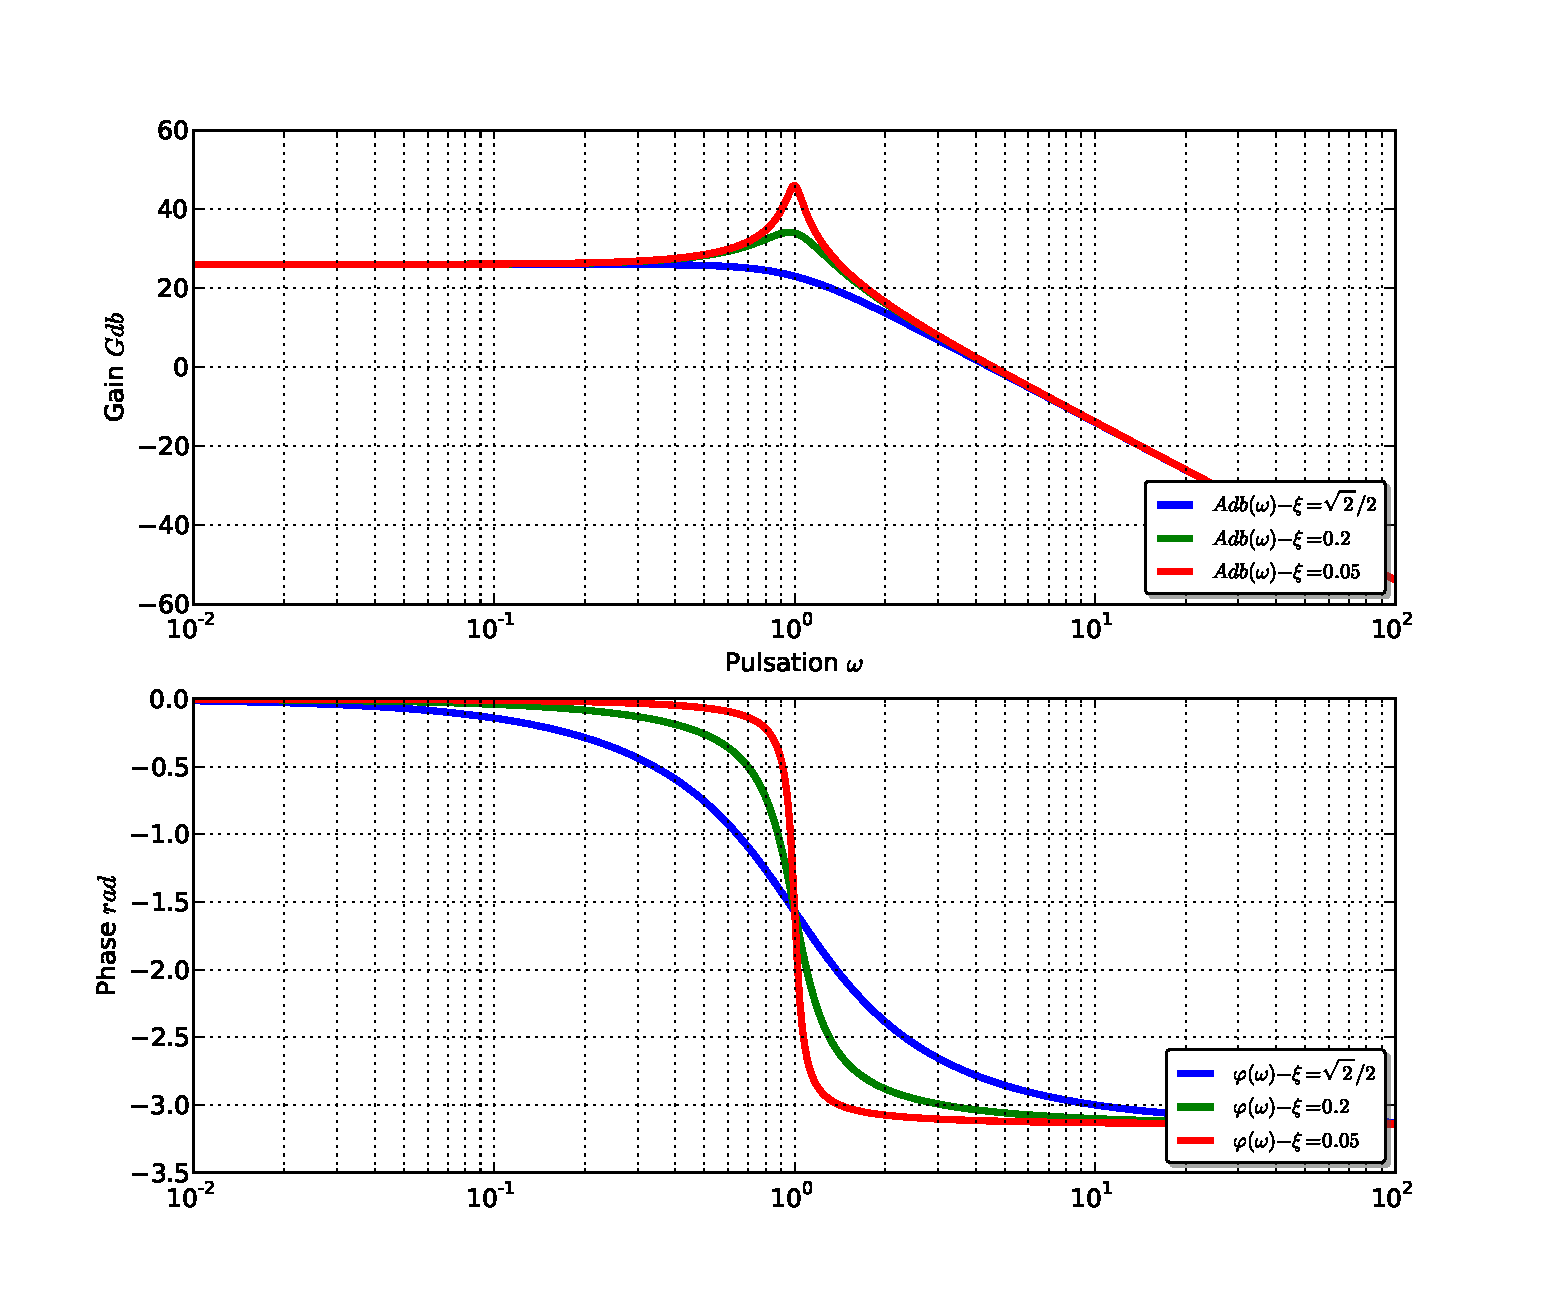
\includegraphics[width=.9\textwidth]{png/ordre2_bode.pdf}

\textit{Diagramme de Bode -- $H(p)=\dfrac{20}{1+ \dfrac{2\xi}{1}p+\dfrac{p^2}{1^2}}$}
\end{center}

\begin{resultat}
\textbf{Phénomène de résonance}

Le phénomène de résonance s'observe lorsque $\xi<\dfrac{\sqrt{2}}{2}$.

La pulsation de résonance est inférieure à la pulsation propre du système :
$$
\omega_r = \omega_0\sqrt{1-2\xi^2}
$$

\`A la résonance, l'amplitude maximale est de 
$$
A_{max} = \dfrac{K}{2\xi\sqrt{1-\xi^2}}
$$

(Attention, sur le diagramme de Bode, on lit $20\log A_{max}$ lorsque $\omega=\omega_r$.
\end{resultat}
%\end{minipage}\hfill
%\begin{minipage}[c]{.48\linewidth}
%\begin{center}
%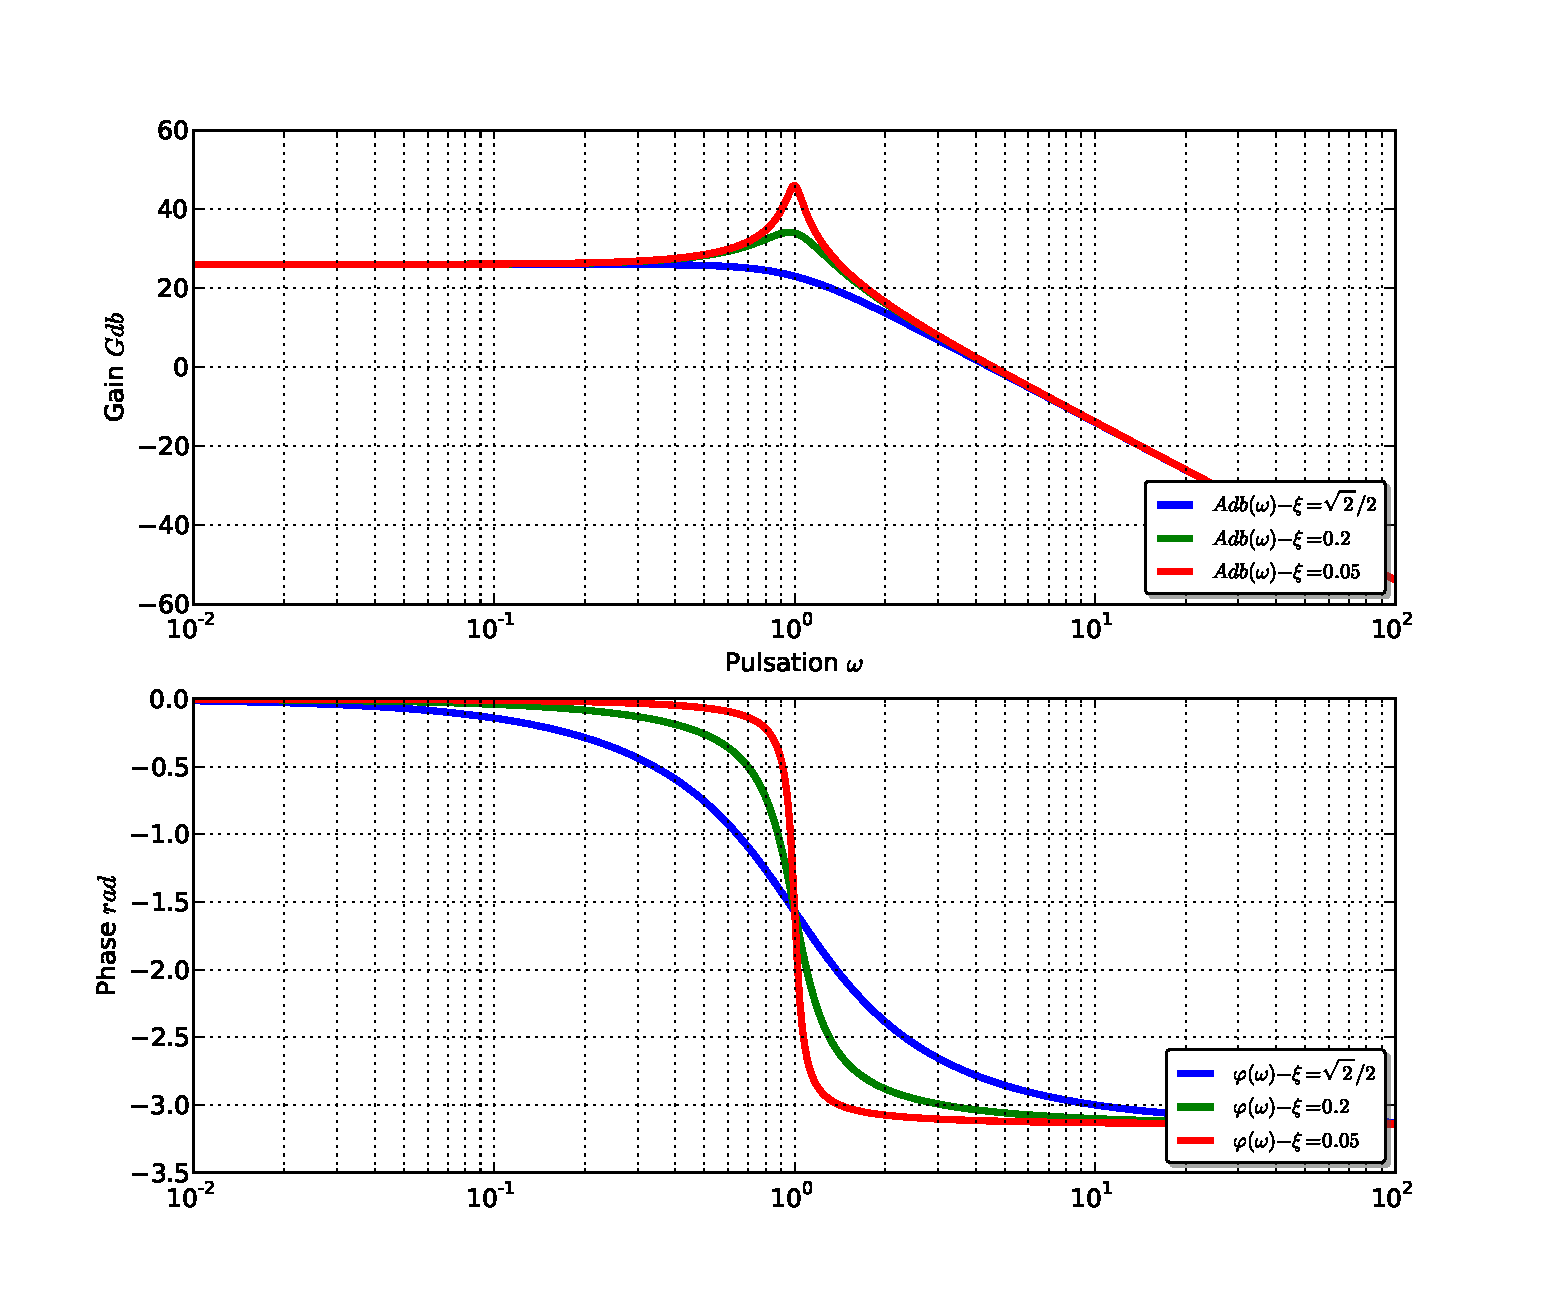
\includegraphics[width=.9\textwidth]{png/ordre2_bode}

%\textit{Diagramme de Bode -- $H(p)=$}
%\end{center}
%\end{minipage}


% \section{Réponse harmonique d'un système asservi}

\begin{thebibliography}{2}
   %\bibitem[1]{cite1} DMU 60 eVo linear, \textit{DMG -- Deckel Maho -- Gildemeiseter}, \url{http://fr.dmg.com}.
   %\bibitem[2]{cite2} Programmation des machines-outils à commande numérique (MOCN), \textit{Étienne Lefur et Christophe Sohier}, École Normale Supérieure de Cachan, \url{http://etienne.lefur.free.fr/}.
\bibitem[1]{cite1} \textit{Jean-Pierre Pupier}, SLCI : Réponse harmonique des systèmes du premier et du second ordre. PTSI -- Lycée Rouvière de Toulon.
   \bibitem[2]{cite2} \textit{Joël Boiron}, SLCI : Étude générale des systèmes fondamentaux du premier et du deuxième ordre. PTSI -- Lycée Gustave Eiffel de Bordeaux.

\end{thebibliography}

\end{document}
 